\section{Overview of the Complexity Zoology Data Set}

This section enumerates the complexity classes, inclusions, and oracle separations
of Complexity Zoology's data set. The data is listed in the same order as in the 
data itself: alphabetically by complexity class, with relations listed under the 
class that appears on the left side of the relation. As a result, many classes are
discussed before the subsection in which they are defined. Some trivial inclusions
are omitted. Statements of equality appear under the less preferred name for the 
class. Large parts of this data set, especially those inclusions that are 
considered to be open, are based on email and in-person communication with Scott 
Aaronson and Lance Fortnow.

Complexity Zoology studies the relationships between complexity classes in six 
different modal worlds: all oracles, all algebraic oracles, some algebraic 
oracle, the random oracle, the trivial oracle, and some oracle. The data set 
would be considered complete when each possible inclusion is settled as true, 
false, or open in each of these six worlds. The current status of the data set is 
shown in Table \ref{data-status}. Note that the trivial world is complete (i.e., 
there are no unknown inclusions).

\begin{table}[]
\begin{tabular}{lllllll}
World:                & P     & D    & O    & UP  & UD   & UU   \\ \hline
All oracles           & 3680  & 9354 & 460  & 20  & 417  & 111  \\
All algebraic oracles & 3022  & 3332 & 326  & 0   & 3918 & 114  \\
Some algebraic oracle & 3022  & 2185 & 0    & 326 & 0    & 5179 \\
Random oracle         & 2435  & 5405 & 1058 & 508 & 156  & 140  \\
Trivial oracle        & 2566  & 2021 & 4725 & 0   & 0    & 0    \\
Some oracle           & 11344 & 2542 & 0    & 156 & 0    & 0   
\end{tabular}
\caption{\label{data-status} The current status of the Complexity Zoology data 
set. This table shows the number of inclusions of each type that exist for each 
world. P indicates \textit{proven}, D indicates \textit{disproven}, O indicates 
\textit{open}, UP indicates \textit{unknown but provable}, and UU indicates 
\textit{unknown with no further data}. The terms \textit{unknown}, 
\textit{provable}, and \textit{disprovable} are explained in Sections 
\ref{zoology-logic} and \ref{extremal-unknowns}.}
\end{table}

\begin{figure}[htb]
  \center{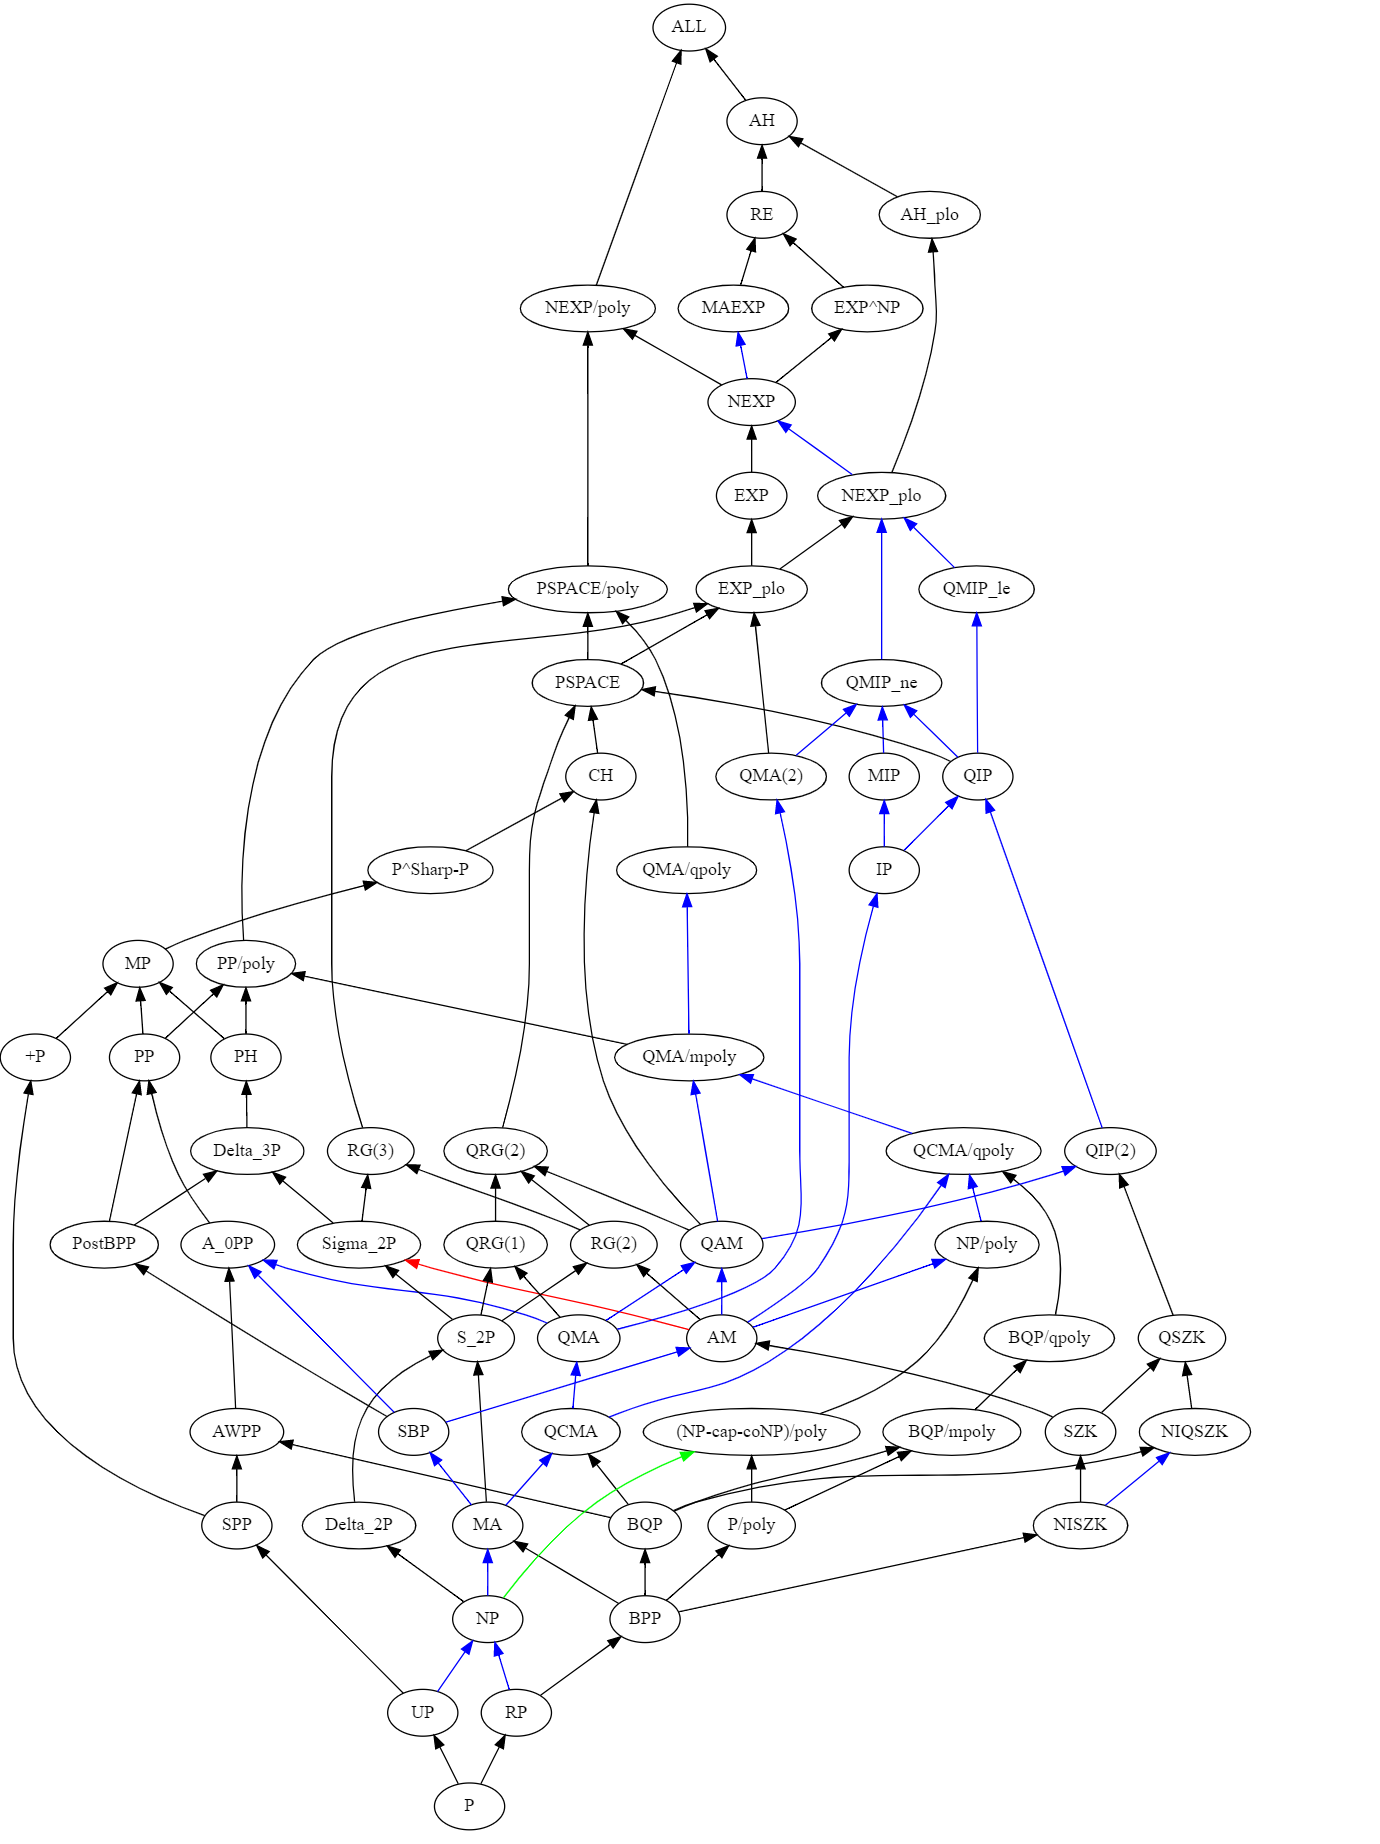
\includegraphics[height=7.7in]
  {all-oracles-full.png}}
  \caption{\label{fig:mini-zoo-inclusion} Inclusions that hold with respect to 
  every oracle. Blue arrows denote containment, black arrows denote symmetric 
  containment, red arrows indicate that the complement of the first class is contained 
  in the second, and green arrows indicate that the intersection of the first class with
  its complement is contained in the second class.}
\end{figure}

\begin{figure}[htb]
  \center{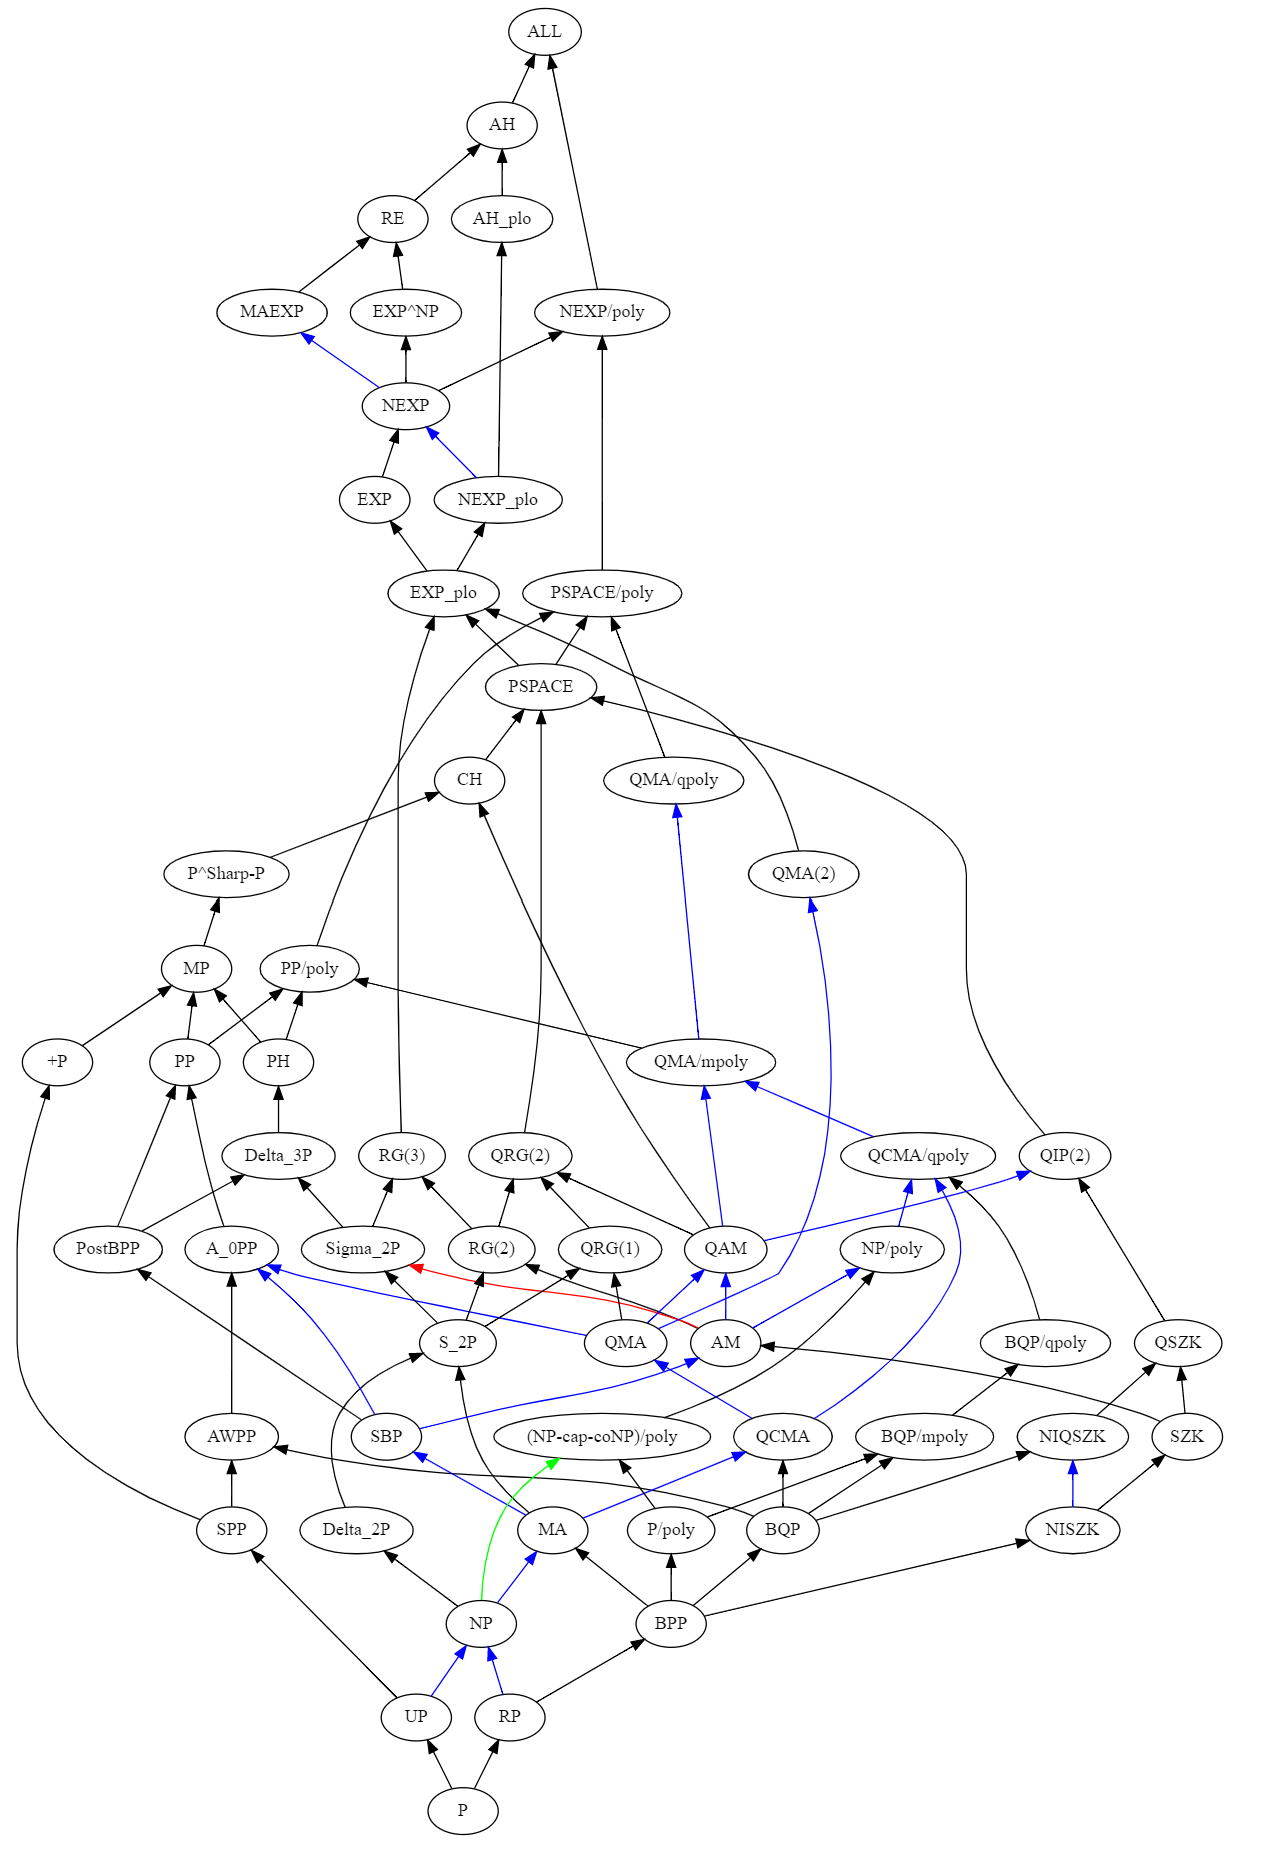
\includegraphics[height=8in]
  {algebraic-oracles-full.png}}
  \caption{\label{fig:mini-zoo-inclusion} Inclusions that hold with respect to 
  all algebraic oracles.}
\end{figure}

\begin{figure}[htb]
  \center{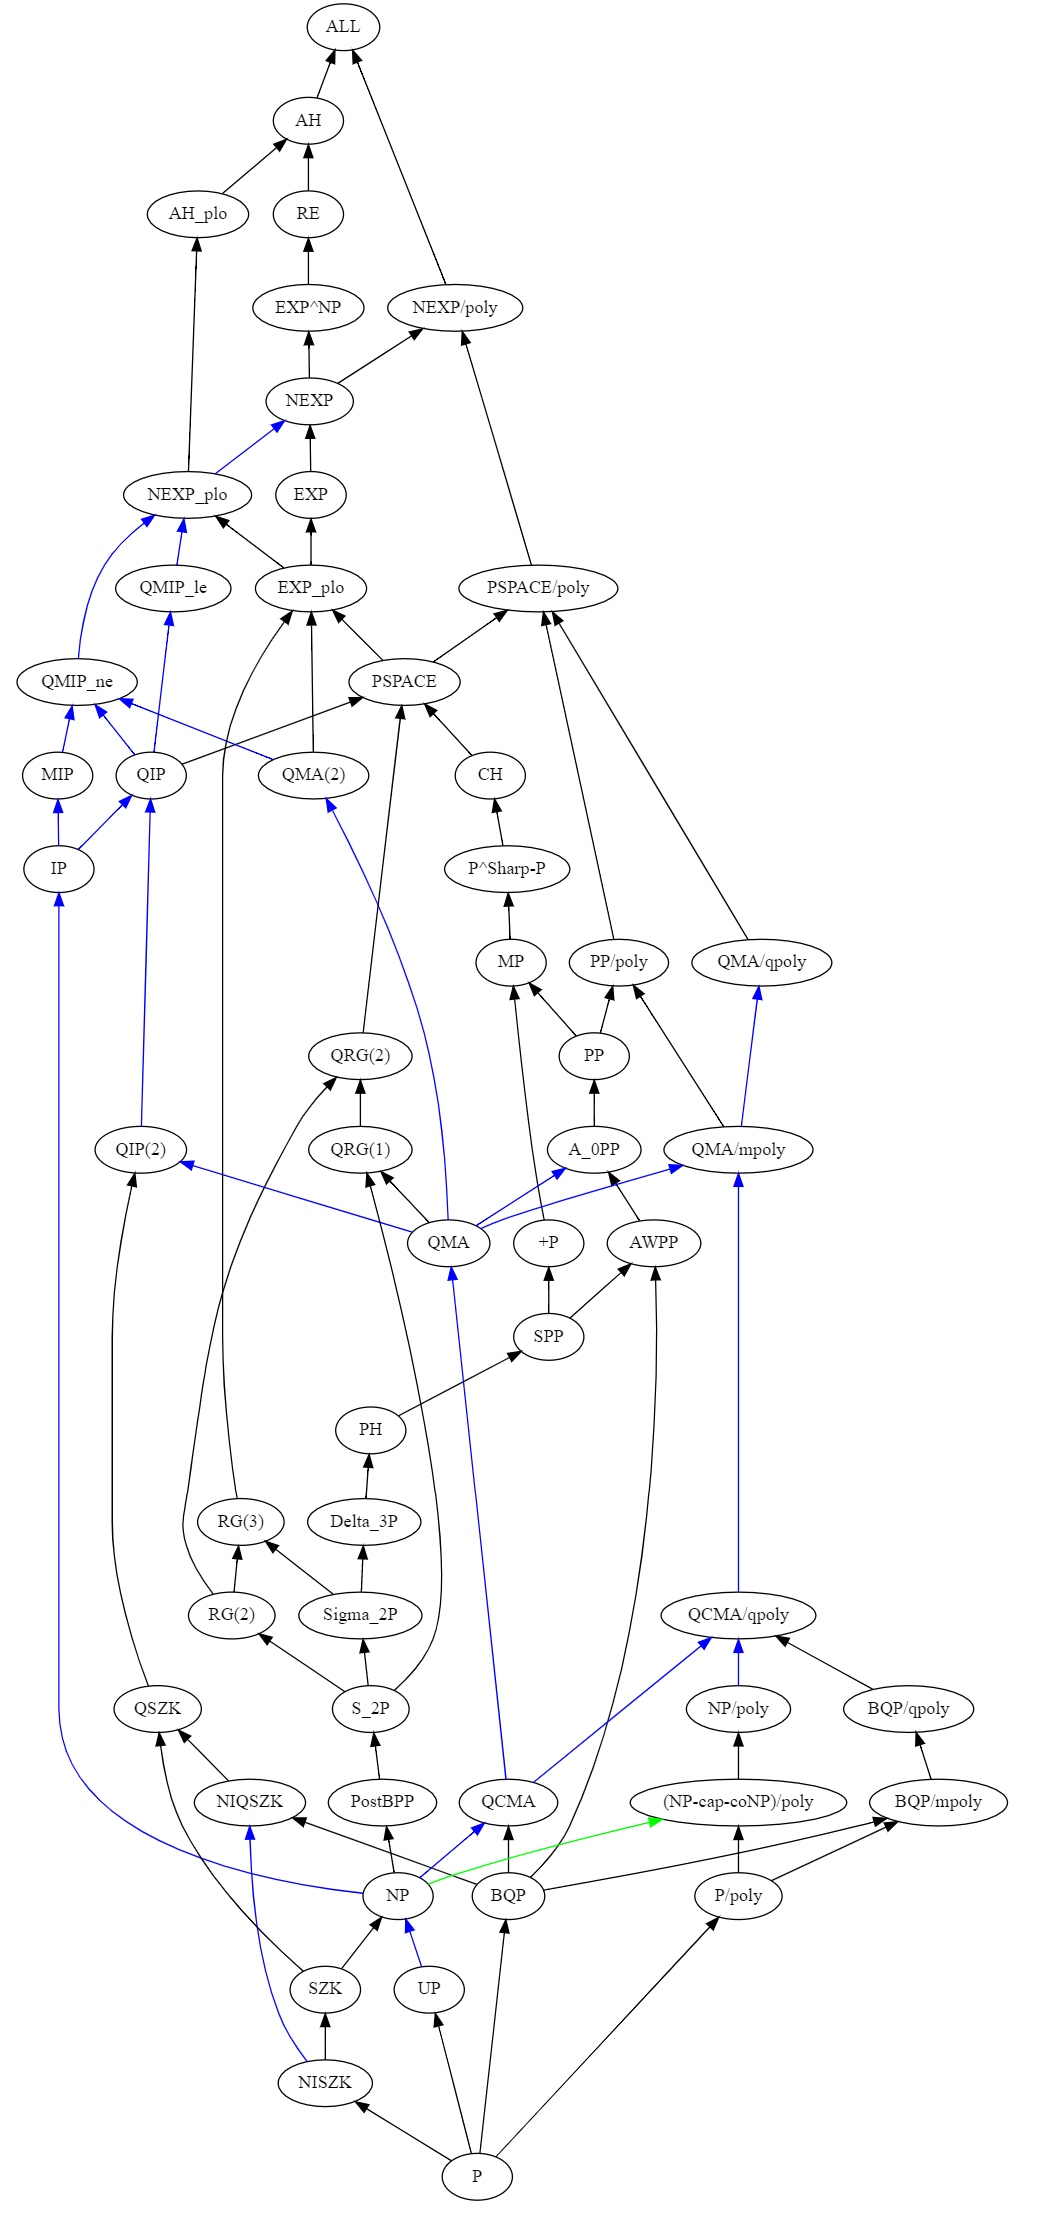
\includegraphics[height=8in]
  {random-oracle-full.png}}
  \caption{\label{fig:mini-zoo-inclusion} Inclusions that hold with respect to 
  the random oracle.}
\end{figure}

\begin{figure}[htb]
  \center{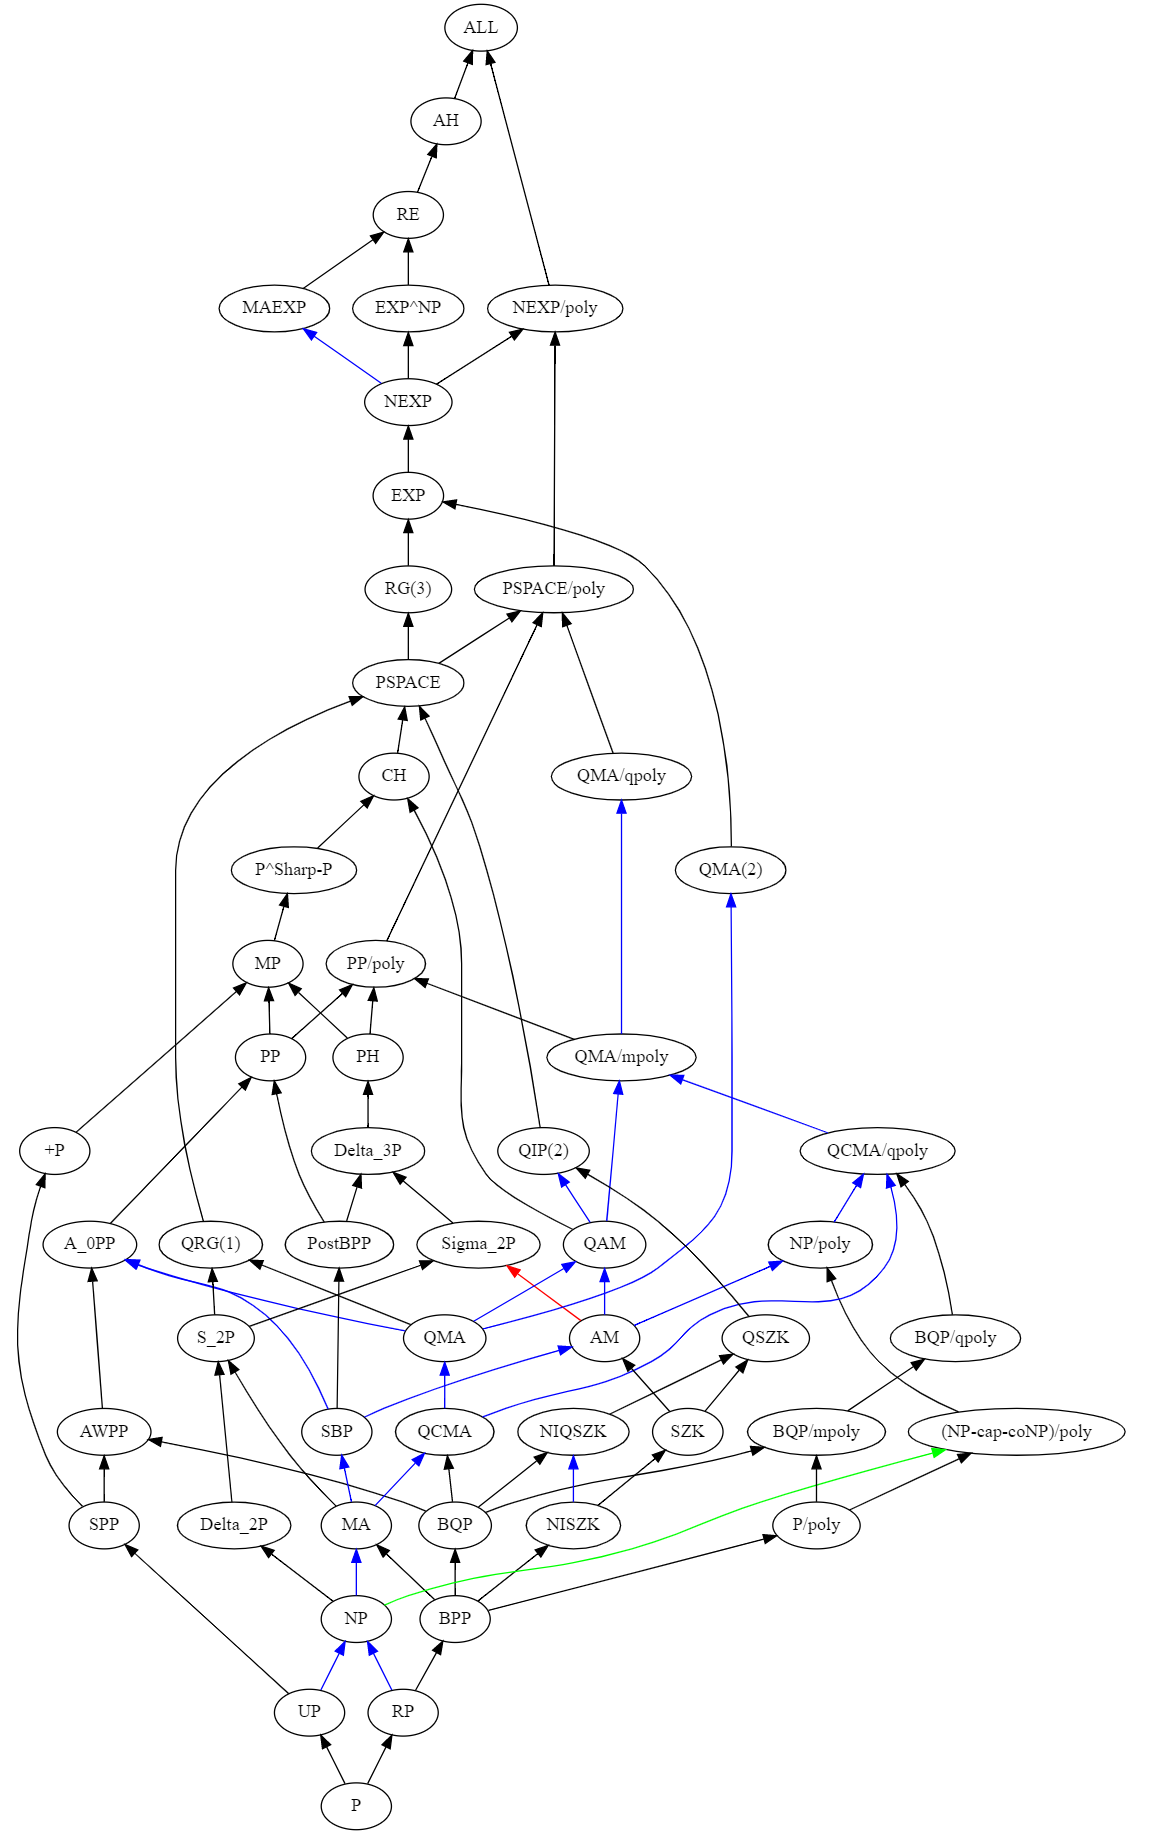
\includegraphics[height=8in]
  {trivial-oracle-full.png}}
  \caption{\label{fig:mini-zoo-inclusion} Inclusions that hold with respect to 
  the trivial oracle (the unrelativized world).}
\end{figure}

\subsection{$\oplus\msf{P}$}

$\oplus\sP$ is the class of languages $\cL$ such that for an $\NP$-machine
$M$ $x\in\cL$ if and only if the computational tree of $M(x)$ has an odd number
of accepting paths. In operator terms, it is equal to $\oplus\cdot\sP$.

$\oplus\sP\subseteq\msf{MP}$ with respect to every oracle \cite{green1995power}.
$\oplus\sP\not\subseteq\msf{PP}/\poly$ with respect to the random oracle, while 
it is open whether this is the case with respect to the trivial oracle.

\subsection{$\msf{A}_0\msf{PP}$}

A function $f:\Sigma^*\ra\Z$ lies in $\msf{GapP}$ if and only if there
exists a polynomial-time Turing machine $M$ and a function $p(n)=\Oh(n^*)$ such 
that for every $x\in\Sigma^*$,
\[
f(x)=|\{y\in\Sigma^{p(|x|)}:M(x,y)=1\}|-|\{y\in\Sigma^{p(|x|)}:M(x,y)=0\}|.
\]
Now $\cL\in\msf{A}_0\msf{PP}$ if and only if there exists a function
$f\in\msf{GapP}$ and a function $g:\Sigma^*\ra\N$ in $\msf{FP}$ such that
\begin{align*}
x\in\cL&\Longrightarrow f(x)>g(x), \\
x\not\in\cL&\Longrightarrow f(x)<g(x)/2.
\end{align*}
Note that a language in $\cL\in\msf{PP}$ can be characterized by the sign of 
some $\msf{GapP}$ function. Since $\msf{GapP}$ is closed under subtraction, it 
follows that $\msf{A}_0\msf{PP}\subseteq\msf{PP}$ for all oracles.

Kuperberg has also shown \cite{kuperberg2009hard} that $\msf{A}_0\msf{PP}$ is equal
to the class $\msf{SBQP}$ of languages $\cL$ such that there exists a 
$\msf{BQP}$-machine $M$ and a function $p(n)=\Oh(n^*)$ such that for all 
$x\in\Sigma^*$,
\begin{align*}
x\in\cL&\Longrightarrow\Pr[M(x)=1]\geq 2^{-p(|x|)}, \\
x\not\in\cL&\Longrightarrow\Pr[M(x)=1]\leq 2^{-p(|x|)-1}.
\end{align*}

\subsection{$\msf{AH}$}

The \textit{arithmetical hierarchy} is analogous to the polynomial hierarchy,
except that $\msf{R}$ and $\msf{RE}$ are the fundamental complexity classes
rather than $\sP$ and $\NP$. Thus, where $\msf{PH}$ is a hierarchy of 
complexity, $\msf{AH}$ is one of computability. For every $n\in\N$, define 
$\Delta_n$, $\Sigma_n$, and $\Pi_n$ by recursion as
follows: $\Delta_0=\Sigma_0=\Pi_0=\msf{R}$, and for every $n\in\N$,
\begin{align*}
\Delta_{n+1}&=\msf{R}^{\Sigma_n}, \\
\Sigma_{n+1}&=\msf{RE}^{\Sigma_n}, \\
\Pi_{n+1}&=\cco\cdot\msf{RE}^{\Sigma_n}.
\end{align*}
Then set $\msf{AH}=\bigcup_{n\in\N}\Sigma_n$.

Since $\msf{R}\subseteq\msf{RE}$ and $\msf{R}$ is a symmetric class it is
immediate that $\Delta_n\subseteq\Sigma_n$ and $\Delta_n\subseteq\Pi_n$ for all
$n\in\N$. Moreover, for $n\geq 1$ we have
\[
\Sigma_n=\msf{RE}^{\Sigma_{n-1}}\subseteq\msf{R}^{\msf{RE}^{\Sigma_{n-1}}}
=\msf{R}^{\Sigma_n}=\Delta_{n+1},
\]
and for $n=0$ we have
\[
\Sigma_0=\msf{R}\subseteq\msf{R}^{\msf{R}}=R^{\Sigma_0}=\Delta_1,
\]
so we also have $\Sigma_n\subseteq\Delta_{n+1}$ and $\Pi_n\subseteq\Delta_{n+1}$
for all $n\in\N$. It follows that
$\msf{AH}=\bigcup_{n\in\N}\Delta_n=\bigcup_{n\in\N}\Pi_n$. Also, just as there 
is an alternating quantifier definition for the polynomial hierarchy, there is 
one for the arithmetical hierarchy. For example, $\cL\in\Sigma_2$ if and only 
there exists a computable relation $R$ such that
\[
x\in\cL\Longleftrightarrow (\exists y)(\forall z)R(x,y,z)
\]
for each $x\in\Sigma^*$.

$\msf{AH}$ is closed under exponential padding: $\msf{AH}=\exppad\cdot\msf{AH}$.

\subsection{$\msf{AH}_{plo}$}\label{ah-plo-subsection}

$\msf{AH}_{plo}$ denotes $\msf{AH}$ with a polynomially-limited oracle
access. The definitions of $\msf{AH}_{plo}$ and $\msf{AH}$ in the
unrelativized case are identical, but $\msf{AH}^f$ and $\msf{AH}_{plo}^f$
have different definitions for an arbitrary oracle $f$.

For $n\in\N$ and an oracle $f:\Sigma^*\ra\Sigma^*$, we define 
$f|_n:\Sigma^*\ra\Sigma^*$ according to the
rule
\[
f|_n(x)=\begin{cases}f(x) &\text{ if }|x|<n, \\
0 &\text{ otherwise}.\end{cases}
\]
then we say that $\cL$ lies in $\msf{RE}_{\msf{plo}}^f$ if and only if there exists an oracle Turing machine $M$ and a function $p(n)=\Oh(n^*)$ such that
\[
x\in\cL\Longrightarrow M\text{ accepts }x\text{ with
}f|_{p(|x|)}\text{-oracle}.
\]
Now we can define $\msf{AH}_{plo}^f$ as we defined $\msf{AH}$: use 
$\msf{RE}_{plo}^f$ and $\msf{R}_{plo}^f=\cocap\cdot\msf{RE}_{plo}^f$ in the 
place of $\msf{RE}$ and $\msf{R}$ in the unrelativized definition of $\msf{AH}$.

$\msf{AH}_{plo}$ is not contained in $\msf{NEXP}/\poly$ and $\msf{RE}$ with 
respect to the random oracle.

Limiting $\msf{AH}$ to polynomial-length oracle queries has the effect of
creating an oracle collapse from $\msf{AH}$ all the way to $\sP$. In fact, we
can prove something even stronger: there exists an oracle relative to which
$\sP=\msf{AH}[poly]$, where $\msf{AH}[poly]$ is a class containing
$\msf{AH}$. 
$\msf{AH}[poly]$ is the class of languages $\cL$ such that there exists a
computable relation $R$ and a function $p(n)=\Oh(n^*)$ such that for every
$x\in\Sigma^*$,
\begin{align*}
x\in\cL\Longleftrightarrow
&(Q_1y_1\in\Sigma^*)\ldots(Q_{p(|x|)}y_{p(|x|)}\in\Sigma^*)
R(x,y_1,\ldots,y_{p(|x|)})\hspace{6pt}\OR \\
&(\bar Q_1y_1\in\Sigma^*)\ldots(\bar Q_{p(|x|)}y_{p(|x|)}\in\Sigma^*)
R(x,y_1,\ldots,y_{p(|x|)}),
\end{align*}
where $Q_k$ is $\forall$ when $k$ is even and $\exists$ when $k$ is odd, and
$\bar Q_k$ is $\exists$ when $k$ is even and $\forall$ when $k$ is odd.

The relativizing inclusion $\msf{AH}\subseteq\msf{AH}[poly]$ is immediate from
the alternating quantifier definition of $\msf{AH}$. Using the same quantifier definition as above, set
\begin{align*}
\mathtt{AHSAT}=&\{\inner{\alpha,x,1^m}:
(Q_1y_1\in\Sigma^*)\ldots(Q_my_m\in\Sigma^*)[M_\alpha(x,y_1,\ldots,y_m)=1])
\text{ or }\\
&(\bar Q_1y_1\in\Sigma^*)\ldots(\bar Q_my_m)\in\Sigma^*)
[M_\alpha(x,y_1,\ldots,y_m)=1])\},
\end{align*}
where $M_\alpha$ denotes the Turing machine that $\alpha$ encodes.
\begin{proposition}
$\mathtt{AHSAT}$ is $\msf{AH}[poly]$-complete.
\end{proposition}
\begin{proof}
To see that $\mathtt{AHSAT}\in\msf{AH}[poly]$, we can simply take $p$ to be the
identity function and $R$ to be the relation
\[
R(\inner{\alpha,x,1^m},y_1,\ldots,y_r)\Longleftrightarrow
r\geq m\AND M_\alpha(x,y_1,\ldots,y_m)=1.
\]
Then $R$ and $p$ witness that $\mathtt{AHSAT}\in\msf{AH}[poly]$ per the
definition.

Now suppose that $\cL\in\msf{AH}[poly]$, and let the relation $R$ and the
function $p(n)=\Oh(n^*)$ witness that $\cL\in\msf{AH}[poly]$. Then, if $\alpha$ is
a code for the Turing machine that computes $R$, we have
\[
x\in\cL\Longleftrightarrow\inner{\alpha,x,1^{p(|x|)}}\in\mathtt{AHSAT}.
\]
Since $p$ is assumed to be time-constructible, the function
$x\mapsto\inner{\alpha,x,1^{p(|x|)}}$ is polynomial-time computable, and so
$\cL$ is polynomial-time reducible to $\mathtt{AHSAT}$. Therefore,
$\mathtt{AHSAT}$ is a complete problem for $\msf{AH}[poly]$.
\end{proof}
Since $\sP\subseteq\msf{AH}[poly]$ relative to any oracle, in particular
$\sP^{\mathtt{AHSAT}}\subseteq\msf{AH}[poly]_{plo}^{\mathtt{AHSAT}}$. Moreover, 
adding an oracle for a problem in $\msf{AH}[poly]$ does not
increase the computational power of $\msf{AH}[poly]_{plo}$, because oracle calls
can be replaced with references to the alternating-quantifier relation 
corresponding to the oracle. So
$\msf{AH}[poly]_{plo}^{\mathtt{AHSAT}}\subseteq\msf{AH}[poly]\subseteq
\sP^{\mathtt{AHSAT}}$. Hence:
\begin{theorem}[Kuperberg]
$\sP^{\mathtt{AHSAT}}=\msf{AH}[poly]_{plo}^{\mathtt{AHSAT}}$.
\end{theorem}

\subsection{$\msf{ALL}$}

$\msf{ALL}$ is the ``complexity'' class of all languages.

While it is not an interesting complexity class in and of itself, $\msf{ALL}$ is
a useful point of reference in the hierarchy of complexity class inclusions. For
instance, it can be helpful to know which classes are immediately below
$\msf{ALL}$ in out hierarchy of inclusions, and it is often a nontrivial theorem
that a particular class is or is not $\msf{ALL}$.

\subsection{$\msf{AM}$}

$\msf{AM}$ is the class of language that can be computed using the
\textit{Arthur-Merlin protocol}. The protocol consists of these steps:
\begin{enumerate}
\item Arthur queries Merlin in an attempt to determine whether $x\in\cL$. Arthur
  is a polynomial-time Turing machine with access to a polynomial-length,
  uniformly random string $y$ of bits. This string is sent to Merlin.
\item Merlin sends a purported proof $z$ (with $|z|$ a polynomial of the length of
  the input) that $x\in\cL$. Merlin is an oracle with access to Arthur's coin 
  tosses, so Merlin can send any $z$ based on the situation.
\item Arthur decides whether to accept the input $x$ based on $\inner{x,y,z}$.
\end{enumerate}
The language $\cL$ is considered to lie in $\msf{AM}$ if the Arthur-Merlin
protocol is likely decide the question of whether $x\in\cL$ correctly. Formally,
we can set $\msf{AM}=\cBP\cdot\msf{NP}$.

Immediately, $\msf{AM}$ is contained in $\msf{QAM}$, $\msf{IP}$, and 
$\msf{RG}(2)$ for every oracle. It is also the case that 
$\msf{AM}\subseteq\Pi_2\sP$ for every oracle \cite{babai1985trading}. On the 
other hand, there is an oracle relative to which $\msf{AM}\not\subseteq\msf{PP}$
\cite{vereschchagin1992power}, and $\msf{AM}\subseteq\msf{NP}$ with respect to 
the random oracle \cite{babai1988arthur}.

\subsection{$\msf{AP}$}

An \textit{alternating Turing machine} is a non-deterministic Turing machine in
which each state is assigned either the symbol $\wedge$ or the symbol
$\vee$. Each configuration in a computational tree involving an alternating
Turing machine can likewise be assigned $\wedge$ or $\vee$ based on the current
state of the machine.

To determine whether an alternating Turing machine $M$ accepts an input $x$,
assign an element of $\Sigma$ to each node in the computational tree according
to the following procedure:
\begin{enumerate}
\item If a configuration $c$ is a halting configuration, set $v(c)=0$ if the
  output is 0 and $v(c)=1$ if the output is 1.
\item If $c$ is an $\wedge$-configuration, assign $v(c)=1$ if $v(c^\prime)=1$
  for each descendant $c^\prime$ of $c$ in the computational tree. Otherwise,
  set $v(c)=0$.
\item If $c$ is an $\vee$-configuration, assign $v(c)=1$ if $v(c^\prime)=1$ for
  some descendant $c^\prime$ of $c$ in the computational tree.
\end{enumerate}
Then, we say that $M$ accepts the input $x$ if and only if
$v(s_{\text{start}})=1$.

$\cL\in\msf{AP}$ if there exists a polynomial-time alternating Turing machine
$M$ such that
\[
x\in\cL\Longleftrightarrow M\text{ accepts }x.
\]
for every $x\in\Sigma^*$.

$\msf{AP}=\msf{PSPACE}$ for every oracle \cite{chandra1981alternation}.

\subsection{$\msf{AWPP}$}

$\msf{AWPP}$ is the class of ``almost wide'' $\msf{PP}$ problems. For a 
polynomial-time Turing machine $M$ and a function $p(n)=\Oh(n^*)$, define
\[
d_{M,p}(x)=|\{y\in\Sigma^{p(|x|)}:M(x,y)=0\}|-|\{y\in\Sigma^{p(|x|)}:M(x,y)=1\}|
\]
for each $x\in\Sigma^*$. $\cL\in\msf{AWPP}$ if there exists a polynomial-time 
Turing machine $M$, a function $f:\Sigma^*\ra\N$, and functions 
$p(n),q(n)=\Oh(n^*)$ such that
\begin{align*}
x\in\cL&\Longrightarrow(1-2^{-q(|x|)})f(x)\leq d_{M,p}(x)\leq f(x), \\
x\not\in\cL&\Longrightarrow 0\leq d_{M,p}(x)\leq 2^{-q(|x|)}f(x).
\end{align*}
$\msf{AWPP}\subseteq\msf{A}_0\msf{PP}$ for all oracles \cite{vyalyi2003qma}.

\subsection{$\msf{BPP}$}

This is the class of languages computable in polynomial time using randomness, 
where the computer is correct with a probability of at least $2/3$. In other 
words, $\msf{BPP}=\cBP\cdot\sP$.

It is contained in $\msf{BQP}$, $\msf{MA}$, $\msf{NISZK}$,  and $\msf{SZK}$ with
respect to every oracle. $\msf{BPP}\subseteq\Sigma_2$ for every oracle 
\cite{lautemann1983bpp}, but there is an oracle relative to which 
$\msf{BPP}\not\subseteq\Delta_2\sP$. In the random oracle world, $\sP=\msf{BPP}$
\cite{bennett1981relative}. $\msf{BPP}\not\subseteq\Delta_2\sP$ is open in the 
unrelativized world.

\subsection{$\msf{BPP}_{path}$}

$\msf{BPP}_{path}$ is the original name for $\msf{PostBPP}$, or $\msf{BPP}$ with 
postselection. It was originally defined as the class of all languages $\cL$ such 
that there exists a non-deterministic polynomial-time Turing machine $M$ and a 
threshold $\epsilon>0$ such that for every $x\in\Sigma^*$, the number of paths for
which $M(x)=\cL(x)$ is at least $(1/2+\epsilon)\cdot T(x)$, where $T(x)$ is the 
total number of computational paths of $M$ with input $x$  
\cite{han1997threshold}.

\subsection{$\msf{BQP}$}

Informally, $\msf{BQP}$ is the set of languages that can be computed efficiently
using a quantum computer. A quantum computer can be modeled by a uniform family 
of quantum circuits or a quantum Turing machines whose configurations can be 
quantum states.

$\msf{BQP}\subseteq\msf{BQP}/\msf{mpoly}$ is immediate. $\msf{BQP}$ is also 
contained in $\msf{AWPP}$ for every oracle \cite{fortnow1998complexity}, as well
as $\msf{NIQSZK}$, $\msf{QCMA}$, and $\msf{QSZK}$. There exist oracles relative 
to which $\msf{BQP}$ is not contained in $\oplus\sP$, $\msf{PH}$, $\msf{MA}$ 
\cite{watrous2000succinct}, $\NP/\poly$, $\msf{PostBPP}$ \cite{aaronson2010bqp} 
\cite{chen2016note},
and $\msf{SZK}$ \cite{childs2003exponential}. Recently, $\msf{PH}$ was added to 
this list of oracle separations \cite{raz2018oracle}.

In the random oracle world, the following inclusions are open:
\[
\msf{BQP}\subseteq\msf{BPP},\msf{IP},\msf{MIP},\sP,\msf{PH},\oplus\sP,\NP/\poly.
\]
It is also open whether $\msf{BQP}$ is contained in $\msf{PH}$ and $\NP/\poly$ 
in the unrelativized world and whether there exists an oracle such that 
$\msf{BQP}\not\subseteq\msf{MIP}$.

\subsection{$\msf{BQP}/\msf{mpoly}$}\label{bqp-mpoly}

$\msf{BQP}/\msf{mpoly}$ is $\msf{BQP}$ with ``Merlinized'' polynomial advice.
\begin{definition}
$\cL\in\msf{BQP}/\msf{mpoly}$ if there exists a $\msf{BQP}$-machine $M$ and a
polynomial-length advice function $f:\N\ra\Sigma^*$ such that
\[
x\in\cL\Longleftrightarrow\Pr[M(x,f(n))=\cL(x)]\geq 2/3.
\]
\end{definition}
The advice is ``Merlinized'' in the sense that the probability threshold of $\geq 
2/3$ need only be observed when the advice is good, just as Arthur does not need 
to satisfy the probability gap when Merlin gives a poor argument in the 
Arthur-Merlin protocol.

$\msf{BQP}/\msf{mpoly}$ is also the class of languages that can be computed using 
some family of polynomial-sized quantum circuits.

$\msf{BQP}/\msf{mpoly}\subseteq\msf{BQP}/\msf{qpoly},\msf{QMA}/\msf{qpoly}$ for 
every oracle.

\subsection{$\msf{BQP}/\msf{qpoly}$}

$\msf{BQP}/\msf{qpoly}$ is $\msf{BQP}$ with a polynomial amount of quantum 
advice. This means that, rather than a classical advice string, a 
$\msf{BQP}$-machine is given an advice string that 
exists in a state of superposition. That is, the advice string takes the form 
$\sum_s\alpha_s\ket{s}$, where the sum is over polynomial-length strings in 
$\Sigma$.

It is immediate that $\msf{BQP}/\msf{qpoly}\subseteq\msf{QCMA}/\msf{qpoly}$ 
relative to every oracle. In fact, Aaronson and Drucker have shown that 
$\msf{BQP}/\msf{qpoly}\subseteq\msf{QCMA}/\msf{mpoly}$ 
\cite{aaronson2010characterization}. The relationship between classical and quantum
advice in the case of $\msf{BQP}$ is uncertain: it is unknown whether 
$\msf{BQP}/\msf{qpoly}$ is any larger than $\msf{BQP}/\msf{mpoly}$ 
\cite{aaronson2007quantum}.

\subsection{$\msf{BQPSPACE}$}

This is the class of languages computable by a \textit{quantum Turing machine} 
using a polynomial amount of space. A quantum Turing machine is a Turing machine 
that includes a quantum tape on which qubits can be recorded, as well as a finite 
register for performing measurements. As with other non-deterministic versions of 
$\msf{PSPACE}$ (see Subsections \ref{npspace-subsection} and 
\ref{ppspace-subsection}), $\msf{BQPSPACE}$ is equal to $\msf{PSPACE}$ for every 
oracle \cite{watrous2003complexity}.

\subsection{$\msf{CH}$}

The \textit{counting hierarchy} is the class that results from an infinite stack
of $\msf{PP}$-oracles. If $C_0\sP=\sP$ and $C_{k+1}\sP=\msf{PP}^{C_k\sP}$ for 
each $k\in\N$, then $\msf{CH}=\bigcup_kC_k\sP$. The classes $\sP^{C_k\sP}$ are 
clearly inside $\msf{CH}$, and so $\msf{CH}=\sP^{\msf{CH}}$ for every oracle. 
Moreover, because $\msf{PP}\subseteq\msf{PSPACE}$, and because giving 
$\msf{PSPACE}$ access to an oracle that is already inside $\msf{PSPACE}$ does 
not increase the power of the class, we also have the relativizing inclusion 
$\msf{CH}\subseteq\msf{PSPACE}$.

It is unknown whether $\msf{CH}\subseteq\sP^{\#\sP}$ (since 
$\sP^{\#\sP}=\sP^{\msf{PP}}$, this would imply that the counting hierarchy 
collapses) relative to a random oracle, and indeed whether there is any oracle 
relative to which the counting hierarchy does not collapse.

\subsection{$\cocap\cdot\msf{RE}$}

The class $\cocap\cdot\msf{RE}=\msf{RE}\cap\co\msf{RE}$ is equal to $\msf{R}$, 
the class of recursive decision problems. $\msf{RE}$ is the class of languages 
that a computer can enumerate the elements of. If a computer can enumerate the 
elements of a language as well as its complement, then the computer can decide 
whether $x$ lies in the language by enumerating the language and its complement 
until it is revealed where $x$ lies.

\subsection{$\cocap\cdot\msf{RP}$}

The intersection of $\msf{RP}$ and $\co\msf{RP}$ is equal to $\msf{ZPP}$ for 
every oracle.

\subsection{$\Delta_2\sP$}

The class $\Delta_2\sP$ is a level of the polynomial hierarchy, defined to be 
$\sP^\NP$. It is therefore contained in $\Sigma_2\sP=\NP^{\NP}$. Less obviously,
$\Delta_2\sP$ lies in $S_2\sP$ relative to every oracle 
\cite{russell1998symmetric}. While it is unknown whether 
$\Delta_2\sP\subseteq\msf{PP}$ in the unrelativized world, there exists an 
algebraic oracle relative to which $\Delta_2\sP\subseteq\msf{PP}$ 
\cite{aaronson2009algebrization}. $\Delta_2\sP$ is outside $\msf{PostBPP}$ 
relative to the random oracle.

\subsection{$\Delta_3\sP$}

This class is $\sP^{\Sigma_2\sP}$, another level of the polynomial hierarchy. It
is unknown whether $\Delta_3\sP\subseteq\msf{PostBPP}$ relative to the trivial 
oracle.

\subsection{$\msf{EXP}$}

This is the class of languages that can be decided in exponential time. It can 
be succinctly defined as $\exppad\cdot\sP$. By the time hierarchy theorem, 
$\msf{EXP}\not\subseteq\sP$ relative to every oracle, but there is an oracle 
relative to which $\msf{EXP}=\msf{ZPP}$ \cite{Heller1984}, as well as an oracle 
relative to which $\msf{EXP}=\cocap\cdot\msf{UP}$. In the unrelativized world, 
it is unknown whether either of these equalities is true.

\subsection{$\msf{EXP}^\NP$}

This class is $\bigcup_{f\in\NP}\msf{EXP}^f$, or $\msf{EXP}$ relative to an 
$\msf{NP}$-oracle. (It can also be defined to be $\msf{EXP}^{\mathtt{SAT}}$, or 
any other $\NP$-complete problem.) Since $\msf{EXP}=\exppad\cdot\sP$, it follows
that $\msf{EXP}^\NP=\exppad\cdot\Delta_2\sP$. There exist oracles relative to 
which this class is equal to $\msf{BPP}$ \cite{buhrman2000randomness} and 
$\msf{SPP}$. The time hierarchy theorem relativizes, so 
$\msf{EXP}^\NP\not\subseteq\Delta_2\sP$ for every oracle. Additionally, 
$\msf{EXP}^\NP\not\subseteq\msf{NEXP}$ in the random oracle world.

In the unrelativized world, the inclusions 
$\msf{EXP}^\NP\subseteq\msf{NEXP}/\poly,\msf{BPP},\msf{SPP}$ are open.

\subsection{$\msf{EXP}_{plo}$}

As with $\msf{AH}_{plo}$, $\msf{EXP}_{plo}$ is equal to $\msf{EXP}$ in the 
unrelativized world, while relative to an oracle, the oracle calls are limited 
in length to a polynomial of $|x|$ for the input $x$.

\subsection{$\msf{IP}$}

An \textit{interactive proof protocol} is an interaction between a probabilistic
polynomial-time verifier and a deterministic prover with infinite computational 
power. The prover can compute any function, but unlike the Arthur-Merlin 
protocol, the prover does not know the random bits that the verifier uses in his
computations. The verifier attempts to determine whether the input $x$ lies in a
given language $\cL$ within a number of rounds that is a polynomial of $|x|$. 
The language lies in $\msf{IP}$ if and only if the protocol is 
\textit{complete}, meaning that if $x\in\cL$ then the verifier can be convinced 
of this fact with a probability of at least $2/3$, and \textit{sound}, meaning 
that if $x\not\in\cL$ then the verifier can be convinced that $x\in\cL$ with a 
probability of at most $1/3$.

While the prover has the power to determine even uncomputable functions, to 
determine the optimal strategy for the prover, given an input $x$, only a 
$\msf{PSPACE}$-machine is necessary. Using a polynomial-space computation, the 
prover can simulate as many interactions with the prover as needed. Therefore, 
$\msf{IP}\subseteq\msf{PSPACE}$ relative to every oracle.

$\msf{IP}$ is also contained in its generalizations $\msf{QIP}$ and $\msf{MIP}$.
There is an oracle relative to which $\cocap\cdot\msf{IP}\not\subseteq\msf{PH}$ 
\cite{aiello1990power}. Open problems in the random oracle world include whether
$\cocap\cdot\msf{IP}$ is contained in $\msf{PP}/\poly$, $\msf{QMA}/\msf{qpoly}$,
$\msf{CH}$, or $\msf{QMA}(2)$.

\subsection{$\msf{IPP}$}

This class is the unbounded version of $\msf{IP}$. More precisely, the 
completeness and soundness conditions are weakened so that when $x\in\cL$, the 
prover can convince the verifier to accept with a probability of at least $1/2$,
while if $x\not\in\cL$, then in all circumstances the verifier accepts with a 
probability of at most $1/2$. $\msf{IPP}=\msf{PSPACE}$ with respect to every 
oracle \cite{chang1994random}.

\subsection{$\msf{MA}$}

The Merlin-Arthur protocol is similar to the Arthur-Merlin protocol, except that
Merlin sends Arthur a message without knowing Arthur's randomized bits, and 
Arthur decides whether to accept that the input $x$ lies in the language $\cL$ 
using a polynomial-time randomized algorithm. As with many other interaction 
protocols, $\cL\in\msf{MA}$ if and only only if $x\in\cL$ implies that Arthur 
can be persuaded that $x\in\cL$ with probability $\geq 2/3$, while $x\not\in\cL$
implies that Arthur can be persuaded that $x\in\cL$ with probability $\leq 2/3$.

$\msf{MA}\subseteq\msf{QCMA},\msf{SBP}$ relative to every oracle. It is also the
case that $\msf{MA}\subseteq\msf{S}_2\sP$ relative to every oracle 
\cite{russell1998symmetric}. In the unrelativized world, the inclusion 
$\cocap\cdot\msf{MA}\subseteq(\NP\cap\co\NP)/\poly$ is open.

\subsection{$\msf{MAEXP}$}

The class $\msf{MAEXP}$ is the class of languages computable using the 
Merlin-Arthur protocol, where Arthur has exponential computational power. In 
operator terms, $\msf{MAEXP}=\exppad\cdot\msf{MA}$. $\msf{MA}$ is strictly 
contained in $\msf{MAEXP}$ relative to every oracle.

There exist oracles relative to which $\msf{MAEXP}$ is contained in $\oplus\sP$,
$\Delta_2\sP$, and $\sP/\poly$, while in the unrelativized world, 
$\cocap\cdot\msf{MAEXP}\not\subseteq\sP/\poly$ 
\cite{buhrman1998nonrelativizing}. In fact, 
$\cocap\cdot\msf{MAEXP}\not\subseteq\sP/\poly$ relative to every algebraic 
oracle \cite{aaronson2009algebrization}. Relative to the trivial oracle, it is 
open whether $\msf{MAEXP}$ is contained in $(\NP\cap\co\NP)/\poly$, $\msf{BQP}$,
$\Delta_2\sP$, $\msf{SPP}$, $\cocap\cdot\msf{NISZK}$, or $\cocap\cdot\msf{SBP}$.

\subsection{$\msf{MIP}$}

An interactive proof protocol can involve multiple provers. In the class 
$\msf{MIP}$, there are two provers and one verifier. As in $\msf{IP}$, the 
verifier is a polynomial-time probabilistic Turing machine and the provers have 
infinite computing power; however, the provers are not allowed to communicate 
with each other.

$\msf{MIP}$ is contained in $\msf{NEXP}_{plo}$ and its quantum counterpart 
$\msf{QMIP}_{ne}$ relative to every oracle. Open questions include whether  
$\msf{MIP}\subseteq\cco\cdot\msf{MAEXP}$ for every oracle, whether 
$\msf{MIP}\subseteq\cco\cdot\msf{NEXP}$ for the random oracle, and whether 
$\cocap\cdot\msf{MIP}\subseteq\msf{EXP}$ for all oracles and for the random 
oracle.

\subsection{$\msf{MP}$}

For $x\in\Sigma^*$, denote by $x(k)\in\Sigma$ the bit in $x$ at position $k$ 
(indexing from zero). Then, we say $\cL\in\msf{MP}$ if and only if there exists 
$f\in\#\sP$ and a polynomial-time computable $g:\Sigma^*\ra\N$ such that 
$\cL(x)=f(x)(g(x))$ for every $x\in\Sigma^*$. $\msf{MP}$ stands for ``middle 
bit,'' because it can be assumed that $|f(x)|$ is always odd and that 
$g(x)=\frac{1}{2}(|f(x)|-1)$ \cite{green1995power}.

$\msf{MP}$ is contained in $\sP^{\#\sP}$ relative to every oracle, since 
$\sP^{\#\sP}$ can use a $\#\sP$-oracle to determine the middle bit of a function
in $\#\sP$.

\subsection{$\msf{NEXP}$}

This class is the non-deterministic counterpart to $\msf{EXP}$; it can be 
defined to be $\exppad\cdot\NP$. Like $\NP$, it is distinct from its complement 
with respect to an oracle constructed via the password argument. Additionally, 
$\cocap\cdot\msf{NEXP}\not\subseteq\NP$ with respect to every oracle by a 
diagonalization argument.

There exists an oracle relative to which $\msf{NEXP}\subseteq\oplus\sP$ 
\cite{aaronson2006oracles}. In the unrelativized world, the inclusions 
$\msf{NEXP}\subseteq\msf{SPP}$ and $\msf{NEXP}\subseteq\cco\cdot\msf{MAEXP}$ are 
open.

\subsection{$\msf{NEXP}_{plo}$}

This class is identical to $\msf{NEXP}$, except that oracle calls are limited in
length to a polynomial of $|x|$ for input $x$. It is contained in $\msf{MIP}$ 
\cite{aaronson2009algebrization} and $\msf{QMIP}_{le}$ \cite{ito2012multi} with 
respect to all algebraic oracles. The question of whether 
$\msf{NEXP}_{plo}\subseteq\msf{MP}$ relative to every oracle is open.

\subsection{$\msf{NEXP}/\poly$}

Naturally, $\msf{NEXP}/\poly$ is defined to be $\cpoly\cdot\msf{NEXP}$. The 
question of whether $\msf{NEXP}/\poly\subseteq\sP/\poly$ in the unrelativized 
world is open.

\subsection{$\msf{NIQSZK}$}

This class is the non-interactive version of $\msf{QSZK}$, just as $\msf{NISZK}$
is the non-interactive version of $\msf{SZK}$. Accordingly, it lies in 
$\msf{QSZK}$ for every oracle. The inclusions 
\[
\cocap\cdot\msf{NIQSZK}\subseteq\msf{CH},\msf{PP}/\poly,\msf{QMA}/\msf{qpoly}
\]
are open with respect to the trivial oracle.

\subsection{$\msf{NISZK}$}
There is a modified version of the statistical zero-knowledge protocol in which 
interaction between the prover and the verifier is disallowed. More precisely, a
language lies in $\msf{NISZK}$ if and only if the language can be computed using
a statistical zero-knowledge protocol, with the additional constraints that the 
prover and verifier share a single randomly generated string as the source of 
their randomness, and the only communication allowed between the two parties is 
a single message from the prover to the verifier.

There exist oracles relative to which 
$\cocap\cdot\msf{NISZK}\not\subseteq\msf{PP}$ \cite{bouland2017power} and 
$\cocap\cdot\msf{NISZK}\not\subseteq\msf{BQP}/\msf{qpoly}$. Unlike $\msf{SZK}$, 
there is an oracle which $\msf{NISZK}$ is distinct from its complement 
\cite{lovett2017impossibility}. It is open whether 
$\msf{NISZK}\subseteq\msf{NIQSZK}$ in either the world of all oracles or in the 
unrelativized world. The inclusions
\[
\cocap\cdot\msf{NISZK}\subseteq\msf{BQP}/\msf{qpoly},\msf{PP},\msf{QMA}(2),
\msf{QRG}(1),(\NP\cap\co\NP)/\poly
\]
are likewise open in the unrelativized world.

\subsection{$\NP$}

The class of languages that can be computed in non-deterministic polynomial time
can, naturally, be defined to be $\cN\cdot\sP$. It is immediate that 
$\NP\subseteq\msf{MA}$ for every oracle, since $\NP$ is precisely the result of 
the Merlin-Arthur protocol with a deterministic Arthur. Put another way, $\NP$ 
is the class of languages $\cL$ such that if $x\in\cL$, then there is a proof of
this fact that a computer can check in time $p(|x|)$ for some $p(n)=\Oh(n^*)$.

As it is one of the most thoroughly studied complexity classes, there are many 
known oracle separations involving $\NP$. With respect to the random oracle, 
$\NP\not\subseteq\msf{UP}$ \cite{beigel1989relativized} and 
$\NP\not\subseteq\msf{BQP}$ \cite{bennett1997strengths}. There exist oracles 
relative to which $\NP\cap\co\NP\not\subseteq\msf{BQP}$ 
\cite{bennett1997strengths}, $\NP\not\subseteq\msf{BQP}/\msf{qpoly}$ 
\cite{aaronson2004limitations}, $\NP\not\subseteq\cco\cdot\msf{IP}$, 
$\NP\cap\co\NP\not\subseteq\msf{AWPP}$, 
$\NP\not\subseteq\cco\cdot\msf{A}_0\msf{PP}$, and there exist algebraic oracles 
relative to which $\NP\not\subseteq\msf{BQP}$ and 
$\NP\not\subseteq\cco\cdot\msf{MA}$ \cite{aaronson2009algebrization}.

In addition to the famous $\NP\subseteq\sP$ and $\NP\subseteq\co\NP$ in the 
unrelativized world, open questions include whether $\NP\cap\co\NP\subseteq\sP$ 
relative to the random oracle, whether $\NP\subseteq\cco\cdot\msf{A}_0\msf{PP}$ 
or $\NP\cap\co\NP\subseteq\msf{AWPP}$ relative to the trivial oracle, and 
whether $\NP\subseteq\cco\cdot\msf{AM}$ relative to every algebraic oracle.

\subsection{$(\NP\cap\co\NP)/\poly$}

As the class's name would suggest, 
$(\NP\cap\co\NP)/\poly=\cpoly\cdot\cocap\cdot\NP$. Complexity Zoology is able to 
determine the place of this class in the inclusion hierarchy automatically 
through the properties of complexity class operators. In the random oracle 
world, the inclusion $(\NP\cap\co\NP)/\poly\subseteq\sP/\poly$ is open.

\subsection{$\NP/\poly$}

Not only is $\NP/\poly=\cpoly\cdot\NP$, but by the same derandomization argument 
used to show $\msf{BPP}\subseteq\sP/\poly$, we also have 
$\NP/\poly=\cpoly\cdot\msf{AM}$.

Since $\NP\subseteq\msf{MA}$, it follows that 
$\NP/\poly\subseteq\msf{QMA}/\msf{mpoly}$ for every oracle. Likewise, 
$\NP/\poly\subseteq\msf{QCMA}/\msf{qpoly}$ for every oracle. On the other hand, 
there is an oracle relative to which 
$\NP/\poly\not\subseteq(\NP\cap\co\NP)/\poly$ \cite{fenner2003oracle}.

\subsection{$\msf{NPSPACE}$} \label{npspace-subsection}

This class is the non-deterministic version of $\msf{PSPACE}$: 
$\msf{NPSPACE}=\cN\cdot\msf{PSPACE}$. However, $\msf{NPSPACE}$ is no larger than
$\msf{PSPACE}$:
\begin{theorem}[Savitch, \cite{savitch1970relationships}]
$\msf{NPSPACE}=\msf{PSPACE}$ for every oracle.
\end{theorem}
\begin{proof}[Proof sketch]
Given a directed graph with a set $V$ of $n$ vertices and a pair of vertices 
$v,w$, write $\STCON(v,w,k)$ if there exists a path of length $\leq k$ connecting 
$v$ to $w$. To check whether $\STCON(v,w,k)$, recursively check whether each 
vertex $x$ lies halfway along a connecting path:
\[
\STCON(v,w,k)\Longleftrightarrow
\bigvee_{x\in V}(\STCON(v,x,\lfloor k/2\rfloor)\AND
\STCON(x,w,\lceil k/2\rceil))\hspace{12pt}(k\geq 2).
\]
The resulting algorithm uses an $\Oh((\log n)^2)$ amount of space.

Thus, given an $\Oh(f(n))$-space non-deterministic algorithm for a language $\cL$,
we check the $2^{\Oh(f(n))}$-vertex computational tree for a path from the 
starting configuration to the accepting configuration, resulting in a 
deterministic $\Oh((f(n))^2)$-space algorithm.
\end{proof}

\subsection{$\sP$}

The class of languages that are computable in polynomial time is the smallest 
class in Complexity Zoology's data set. There are smaller classes studied in 
complexity theory---such as $\msf{L}$, the class of languages that are 
computable using a logarithmic amount of space---$\sP$ is chosen as the bottom 
of the inclusion hierarchy so that, for instance, polynomial-length oracle calls
are allowed.

Since $\sP$ is the smallest class in Complexity Zoology's data set, it has 
relatively few relations in the input file: we have $\sP\subseteq\msf{UP}$ and 
$\sP\subseteq\msf{ZPP}$ relative to all oracles, both of which are immediate 
from the classes involved.

\subsection{$\sP/\poly$}

The class $\sP/\poly=\cpoly\cdot\sP$ is also equal to $\cpoly\cdot\sP$ is also 
equal to $\cpoly\cdot\msf{BPP}$ via the usual derandomization argument. 
$\sP/\poly\subseteq\msf{BQP}/\msf{mpoly}$ for every oracle, since the latter 
class is a generalization of $\sP/\poly$; and $\sP/\poly\not\subseteq\msf{AH}$ 
for every oracle, because $\sP/\poly$ is uncountable while $\msf{AH}$ is 
countable.

\subsection{$\sP^\msf{PP}$}

We have $\sP^{\msf{PP}}=\bigcup_{f\in\msf{PP}}\sP^f$. As was discussed in 
Section \ref{simplified-version}, $\sP^{\msf{PP}}=\sP^{\#\sP}$ for every oracle,
because we can simulate a $\#\sP$-oracle using multiple $\msf{PP}$-oracle calls.
We also have $\sP^{\msf{PP}}\subseteq\msf{PP}^{\msf{PP}}\subseteq\msf{PP}^{\msf{
C}_1\sP}\subseteq\msf{CH}$.

\subsection{$\sP^{\#\sP}$}

We have $\sP^{\#\sP}=\bigcup_{f\in\#\sP}\sP^f$. The inclusion 
$\sP^{\#\sP}\subseteq\msf{MP}$ is open for both the random and trivial oracles.

\subsection{$\msf{PH}$}

The \textit{polynomial hierarchy} is the class that results from an infinite 
hierarchy of $\NP$-oracles. We set $\Sigma_0\sP=\sP$ and 
$\Sigma_{k+1}\sP=\NP^{\Sigma_k\sP}$ for $k\in\N$, as well as 
$\Pi_k\sP=\cco\cdot\Sigma_k\sP$ and $\Delta_0\sP=\sP$, 
$\Delta_{k+1}\sP=P^{\Sigma_k\sP}$. $\msf{PH}$ is contained in $\msf{MP}$ 
\cite{green1995power} and $\msf{PP}/\poly$ with respect to every oracle, as well
as $\msf{SPP}$ with respect to the random oracle \cite{fortnow1999relativized}. 
On the other hand, $\msf{PH}\not\subseteq\Delta_3\sP$ with respect to the random
oracle, and the question of whether $\msf{PH}\subseteq\Delta_3\sP$ unrelativized
is open.

\subsection{$\msf{PostBPP}$}

The definition of this class is similar to that of $\msf{BPP}$, except we allow 
for \textit{postselection}. Let $(M,p)$ be a polynomial-time Turing machine and 
$\Oh(n^*)$-function, respectively,  such that
\[
\Pr_{y\in\Sigma^{p(|x|)}}[M(x,y)=1]>0
\]
for every $x\in\Sigma^*$. Then $\cL\in\msf{PostBPP}$ if and only if there exists
a polynomial-time Turing machine $M^\prime$ such that for all $x\in\Sigma^*$,
\[
\Pr_{y\in\Sigma^{p(|x|)}}[M^\prime(x,y)=\cL(x)|M(x,y)=1]\geq 2/3.
\]
The condition $M(x,y)=1$ effectively allows us to consider 
$\msf{BPP}$-algorithms in which there is an option for the program to 
\textit{quit} before concluding $x\in\cL$ or $x\not\in\cL$. The algorithm is 
considered successful if it has a high probability of reaching the correct 
answer when it does \textit{not} quit.

$\msf{PostBPP}$ is contained in $\Delta_2\sP$ with respect to the random oracle 
and $\Delta_3\sP$ and $\msf{PP}$ with respect to all oracles. The question of 
whether $\msf{PostBPP}\subseteq\Sigma_2\sP$ in the unrelativized world is open.

\subsection{$\msf{PostBQP}$}

This class is the quantum analogue of $\msf{PostBPP}$. For a $\msf{BQP}$-machine
$M$ and input $x$, denote the value of the $k$th qubit of the output by 
$M(x)_k$, $\cL\in\msf{PostBQP}$ if and only if there exists a 
$\msf{BQP}$-machine $M$ such that for every $x\in\Sigma^*$, $\Pr[M(x)_1=1]>0$ 
and
\[
\Pr[M(x)_0=\cL(x)|M(x)_1=1]\geq 2/3.
\]
It has been shown that $\msf{PostBQP}=\msf{PP}$ for every oracle 
\cite{aaronson2005quantum}.

\subsection{$\msf{PP}$}

Define $\msf{PP}$ to be $\cP\cdot\sP$. Like $\msf{BPP}$, $\msf{PP}$ is based on 
a probabilistic model of computation, except that the machine is only required 
to obtain the correct answer with a probability of at least $1/2$.

$\msf{PP}\subseteq\msf{MP}$ with respect to every oracle. Also, 
$\msf{PP}\subseteq\oplus\sP$ with respect to the random oracle \cite{Raz87b}.

\subsection{$\msf{PP}/\poly$}

This class is simply $\msf{PP}$ with polynomial advice: in operator terms, 
$\msf{PP}/\poly=\cpoly\cdot\cP\cdot\sP$.

\subsection{$\msf{PPSPACE}$} \label{ppspace-subsection}

This is a probabilistic version of $\msf{PSPACE}$: 
$\msf{PPSPACE}=\cP\cdot\msf{PSPACE}$. Ladner \cite{ladner1989polynomial} showed 
that $\msf{PPSPACE}=\msf{PSPACE}$, and this result holds with respect to every 
oracle. (In fact, Ladner proved that the functional counterparts of these classes,
$\#\msf{PSPACE}$ and $\msf{FPSPACE}$, are equal.)

\subsection{$\msf{PSPACE}$}

A $\msf{PSPACE}$-machine is a Turing machine in which the number of cells on 
each tape is limited to some $\Oh(n^*)$ function. $\msf{PSPACE}$ is also equal 
to public-coin $\msf{RG}$ \cite{papadimitriou1985games}, so 
$\msf{PSPACE}\subseteq\msf{RG}$ with respect to every oracle.

$\msf{PSPACE}$ is contained in $\msf{IP}$ with respect to any algebraic oracle 
\cite{aaronson2009algebrization} and $\msf{RG}(2)$ in the unrelativized world 
\cite{feige1997making}. $\msf{PSPACE}\not\subseteq\msf{PH}$ with respect to the 
random oracle \cite{Cai:1986:POR:12130.12133}.

As with many important complexity classes, it is an open question whether 
$\msf{PSPACE}$ is any larger than $\sP$ with respect to the trivial oracle. In 
the world of all oracles, the inclusion $\msf{PSPACE}\subseteq\msf{CH}$ is also 
open.

\subsection{$\msf{PSPACE}/\poly$}

This is $\msf{PSPACE}$ with polynomial advice: 
$\msf{PSPACE}/\poly=\cpoly\cdot\msf{PSPACE}$.

\subsection{$\msf{QAM}$}

The \textit{quantum Arthur-Merlin protocol} is the same as the classical 
Arthur-Merlin protocol, except Arthur is a $\msf{BQP}$-machine instead of a 
classical polynomial-time Turing machine, and Merlin provides a quantum 
certificate.

$\msf{QAM}$ is contained is contained in $\msf{CH}$, $\msf{PP}/\poly$, 
$\msf{QIP}$, $\msf{QIP}(2)$, $\msf{QMA}/\msf{mpoly}$, and $\msf{QRG}(2)$ with 
respect to every oracle. In the random oracle world, $\msf{QAM}$ and $\msf{QMA}$
are equal. In the unrelativized world, the inclusion 
$\cocap\cdot\msf{QAM}\subseteq\sP^{\#\sP}$ is open.

\subsection{$\msf{QCMA}$}

The \textit{quantum-classical Merlin-Arthur protocol} is the same as the 
protocol used in $\msf{QMA}$, except that Merlin's proof must be a classical bit
string. It is immediate that $\msf{QCMA}\subseteq\msf{QMA}$ and 
$\msf{QCMA}\subseteq\msf{QCMA}/\msf{qpoly}$ with respect to every oracle. The 
inclusion $\msf{QCMA}\subseteq\cco\cdot\msf{A}_0\msf{PP}$ is open in the random 
oracle world.

\subsection{$\msf{QCMA}/\msf{qpoly}$}

The class $\msf{QCMA}/\msf{qpoly}$ is $\msf{QCMA}$ with a quantum advice 
string, similar to $\msf{BQP}/\msf{qpoly}$. It is contained in 
$\msf{QMA}/\msf{mpoly}$ for every oracle \cite{aaronson2014full}.

\subsection{$\msf{QIP}$}

In the quantum interactive proof protocol, the verifier is a polynomial-time 
quantum computer, and the prover is a quantum computer with unlimited 
computational power, represented formally by a family of quantum circuits with 
no additional restrictions. The verifier and prover exchange quantum messages 
for a number of rounds that is a polynomial of the length of the input.

For every oracle, we have the immediate inclusions
\[
\msf{QIP}\subseteq\msf{QRG},\msf{QMIP}_{le},\msf{QMIP}_{ne},
\]
as well as $\msf{QIP}\subseteq\msf{PSPACE}$ \cite{jain2010qip}.

\subsection{$\msf{QIP}(2)$}

This class is the special case of $\msf{QIP}$ in which two messages are 
exchanged. Of course, $\msf{QIP}(2)\subseteq\msf{QIP}(3)$ for every oracle.

\subsection{$\msf{QIP}(3)$}

The three-message version of $\msf{QIP}$ is equivalent to the version that 
allows a polynomial number of rounds. That is, $\msf{QIP}(3)=\msf{QIP}$ for 
every oracle \cite{marriott2005quantum}.

\subsection{$\msf{QMA}$}

The quantum Merlin-Arthur protocol is the same as the classical Merlin-Arthur 
protocol, but Arthur is a polynomial-time quantum computer, and the proof that 
Merlin sends to Arthur is quantum.

$\msf{SMA}$ is contained in $\msf{QAM}$, $\msf{QMA}(2)$, 
$\msf{QMA}/\msf{mpoly}$, $\msf{QRG}(1)$, and $\msf{SBQP}$ with respect to every 
oracle. It is open whether there exists an oracle relative to which $\msf{QMA}$ 
has a computational advantage over $\msf{QCMA}$. In the unrelativized world, the
inclusions $\msf{QMA}\subseteq\msf{QCMA}$ and 
$\cocap\cdot\msf{QMA}\subseteq\msf{QCMA}/\msf{qpoly}$ are open.

\subsection{$\msf{QMA}(2)$}

In this variant of $\msf{QMA}$, Merlin sends Arthur two unentangled quantum 
messages rather than one. $\msf{QMA}(2)$ is contained in $\msf{EXP}_{plo}$ and 
$\msf{QMIP}_{ne}$ for all oracles. It is open whether there exists an oracle 
making $\msf{QMA}$ and $\msf{QMA}(2)$ distinct or making $\msf{QMA}(2)$ and 
$\msf{QCMA}$ distinct. In the unrelativized world, the inclusions 
$\msf{QMA}(2)\subseteq\sP$, 
$\cocap\cdot\msf{QMA}(2)\subseteq\msf{PSPACE}/\poly$, and 
$\cocap\cdot\msf{QMA}(2)\subseteq\msf{RG}(3)$ are open.

\subsection{$\msf{QMA}/\msf{mpoly}$}

This class is $\msf{QMA}$ with polynomial-length advice, which is ``Merlinized''
in the sense of $\msf{BQP}/\msf{mpoly}$. It is contained in $\msf{PP}/\poly$ and
$\msf{QMA}/\msf{qpoly}$ with respect to every oracle.

\subsection{$\msf{QMA}/\msf{qpoly}$}

This class is $\msf{QMA}$ with polynomial-length quantum advice. It is contained
in $\msf{PSPACE}/\poly$ with respect to every oracle.

Since $\msf{QMA}\subseteq\msf{QCMA}$ is open in the world of all oracles, so is 
$\msf{QMA}/\msf{qpoly}\subseteq\msf{QCMA}/\msf{qpoly}$. In the random oracle 
world, $\msf{QMA}/\msf{qpoly}\subseteq\NP/\poly$ and 
$\cocap\cdot\msf{QMA}/\msf{qpoly}\subseteq\sP/\poly$ are open, and 
$\cocap\cdot\msf{QMA}/\msf{qpoly}\subseteq\msf{PP}/\poly$ is open in the 
unrelativized world.

\subsection{$\msf{QMIP}_{le}$}

$\msf{QMIP}$ and its related classes are defined similarly to $\msf{MIP}$, 
except that there may be a number of provers bounded by a polynomial of the 
length of the input, the verifier is a polynomial-time quantum computer, and the
provers are quantum computers with infinite computational power. Because the 
provers are quantum, they may share entangled qubits before the protocol begins.
The $le$ in $\msf{QMIP}_{le}$ stands for ``limited entanglement;'' here, the 
provers are required to share at most a polynomially limited number of entangled
qubits.

$\msf{QMIP}_{le}\subseteq\msf{NEXP}_{plo}$ with respect to every oracle. The 
inclusions $\msf{QMIP}_{le}\subseteq\msf{IP}$ is open in the world of all 
oracles, as are $\msf{QMIP}_{le}\subseteq\msf{NP}$ and 
$\msf{QMIP}_{le}\subseteq\cco\cdot\msf{NEXP}$ in the random oracle world and 
$\cocap\cdot\msf{QMIP}_{le}\subseteq\msf{EXP}$ in the trivial oracle world.

\subsection{$\msf{QMIP}_{ne}$}

This is defined in the same manner as $\msf{QMIP}_{le}$, except the provers are 
not allowed to share any entangled qubits. 
$\msf{QMIP}_{ne}\subseteq\msf{NEXP}_{plo}$ with respect to every oracle. The 
inclusions $\msf{QMIP}_{ne}\subseteq\NP$ and $\msf{QMIP}_{ne}\subseteq\msf{IP}$ 
are open in the random and all oracle worlds, respectively.

\subsection{$\msf{QRG}$}

This class is the quantum version of $\msf{RG}$, in which the verifier is a 
polynomial-time quantum Turing machine and the prover and disprover are quantum 
computers with infinite computational power. Unlike $\msf{QMIP}$, there are no 
variants of this class based on entangled qubits, because the prover and 
disprover are working against each other and so there is no benefit in sharing 
entangled qubits.

This class equals $\msf{EXP}_{plo}$ with respect to every oracle 
\cite{gutoski2007toward}.

\subsection{$\msf{QRG}(1)$}

$\msf{QRG}(1)$ is $\msf{QRG}$ with the additional limitation that the prover and
disprover can only send one message to the verifier. The verifier sends no 
messages. The class is, of course, contained in the two-round version 
$\msf{QRG}(2)$ with respect to every oracle. In the unrelativized world, it is 
open whether $\msf{QRG}(1)$ is contained in $\msf{CH}$ or $\msf{PP}/\poly$.

\subsection{$\msf{QRG}(2)$}

This class is $\msf{QRG}$ with two rounds: first, the verifier sends separate messages to the prover and disprover, and then the prover and disprover each send one response. The class is immediately contained in $\msf{QRG}$ with respect to 
every oracle, and it is also contained in $\msf{PSPACE}$ with respect to every
oracle.

\subsection{$\msf{QSZK}$}

This is the quantum counterpart to $\msf{SZK}$. The verifier is a 
polynomial-time quantum computer, and the prover is an all-powerful quantum 
computer. As in the classical case, we require that the verifier's view of his 
interaction be statistically indistinguishable from one that the verifier 
could generate himself. The view, in this case, is a transcript of the quantum
states the verifier sends and receives.

$\msf{QSZK}\subseteq\msf{QIP}(2)$ and $\msf{QSZK}\subseteq\msf{PSPACE}$ for all 
oracles. $\msf{QSZK}\subseteq\msf\sP$ and 
$\msf{QSZK}\subseteq\cocap\cdot\msf{NIQSZK}$ in the random oracle world and all 
oracle world world, respectively.

\subsection{$\msf{R}$}

The class $\msf{R}$ is the foundational class of computability theory. It is the
class of all languages $\cL$ such that $\cL(x)=M(x)$ for all $x\in\Sigma^*$ and 
some Turing machine $M$. Since $\msf{R}$ is not limited except by the 
requirement that languages be computable, it absorbs most of the operators used 
in Complexity Zoology: $\oplus$, $\cBP$, $\cP$, $\cN$, $(\sC\mapsto\sP^\sC)$. 
Diagonalization arguments show that it is larger than most of the time-limited 
models of computation.
\[
\msf{R}\not\subseteq\msf{MAEXP},\msf{EXP}^\NP,\msf{NEXP}/\poly
\]
with respect to every oracle.

\subsection{$\msf{RE}$}

$\msf{RE}$ is the set of all recursively enumerable languages. A language is 
\textit{recursively enumerable} if it is the range of a computable function 
$f:\N\ra\Sigma^*$. Equivalently, $\msf{RE}$ is the set of all languages $\cL$ 
such that for every $x\in\cL$,
\[
x\in\cL\Longrightarrow M(x)=1.
\]
The famously non-computable halting problem is in $\msf{RE}$, and therefore 
$\msf{RE}$ and $\msf{R}$ are distinct. Since $\msf{R}=\cocap\cdot\msf{RE}$, it 
follows that $\msf{RE}$ is not a symmetric class \cite{turing1937computable}.

\subsection{$\msf{RG}$}

A \textit{refereed game} involves an interaction between three parties: a 
prover, a disprover, and a verifier. The verifier is a probabilistic 
polynomial-time Turing machine, while the prover and disprover have infinite 
computational power, although they are unable to see the verifier's coin tosses 
and are similarly isolated from each other. The verifier exchanges messages with
the prover and disprover in parallel for a number of rounds that is a polynomial
of the length of the input. When the interaction ends, the verifier decides to 
accept or reject the input. A language lies in $\msf{RG}$ if and only if there 
is a refereed game in which optimal play convinces the verifier of the correct 
answer with a probability of at least $2/3$.

$\msf{RG}=\msf{EXP}_{plo}$ for all oracles.

\subsection{$\msf{RG}(1)$}

This is the version of $\msf{RG}$ that is restricted to one round of 
interaction, in which the prover and disprover 
each send a message to the verifier. The verifier does not send any messages to 
the prover and the disprover. The class is contained in $\msf{QRG}(1)$, and 
$\msf{RG(2)}$ for every oracle, and it is equal to 
$\msf{S}_2\sP$ for every oracle \cite{fortnow2008complexity}.

\subsection{$\msf{RG}(2)$}

This is the version of $\msf{RG}$ that is restricted to two rounds of 
interaction: first, the verifier sends separate 
messages to the prover and the disprover; then the prover and disprover send a 
response to the verifier. It is contained in 
$\msf{PSPACE}$, $\msf{QRG}(2)$, and $\msf{RG(3)}$ for every oracle.

\subsection{$\msf{RG}(3)$}

This is the version of $\msf{RG}$ that is restricted to three rounds of 
interaction. In round one, the prover and 
disprover separately send a message to the verifier. In round two, the verifier 
sends one reply to the prover and one reply to the disprover. Finally, the prover 
and disprover each respond with another message to the verifier.  It is open 
whether $\msf{RG}(3)$ is contained in $\msf{PSPACE}/\poly$ or $\sP$ with respect 
to the trivial oracle.

\subsection{$\msf{RP}$}

$\msf{RP}$ is another probabilistic model of computation. $\cL\in\msf{RP}$ if 
and only if there exists a polynomial-time Turing machine $M$ and a function 
$p(n)=\Oh(n^*)$ such that for every $x\in\Sigma^*$,
\begin{align*}
x\in\cL&\Longrightarrow
\Pr_{y\in\Sigma^{p(|x|)}}[M(x,y)=1]\geq 2/3, \\
x\not\in\cL&\Longrightarrow
\Pr_{y\in\Sigma^{p(|x|)}}[M(x,y)=1]=0.
\end{align*}
$\msf{RP}\subseteq\NP$ is immediate. We can also inflate the probability of 
$M(x,y)=1$ when $x\in\cL$ by running multiple $\msf{RP}$-machines in parallel. 
Therefore, $\msf{RP}\subseteq\msf{BPP}$ as well.

$\msf{RP}\subseteq\NP$ is immediate. We can also inflate the probability of 
$M(x,y)=1$ when $x\in\cL$ by running multiple $\msf{RP}$-machines in parallel. 
Therefore, $\msf{RP}\subseteq\msf{BPP}$ for every oracle as well.

There is an oracle relative to which $\msf{RP}\not\subseteq\co\NP$ and an 
algebraic oracle relative to which $\msf{RP}\not\subseteq\sP$. In the 
unrelativized world, the inclusions $\msf{RP}\subseteq\co\NP$ and 
$\msf{RP}\subseteq\sP$ are both open.

\subsection{$\msf{S}_2\sP$}

$\msf{S}_2\sP$ is the second level of the \textit{symmetric hierarchy}. The 
definition is similar to that of $\Sigma_2\sP$, except that the "no" condition 
is altered to make the class symmetric. $\cL\in\msf{S}_2\sP$ if and only if 
there exists a polynomial-time Turing Machine $M$ and functions 
$p(n),q(n)=\Oh(n^*)$ such that for every $x\in\Sigma^*$,
\begin{align*}
x\in\cL&\Longrightarrow
(\exists y\in\Sigma^{p(|x|)})(\forall z\in\Sigma^{q(|x|)})[M(x,y)=1], \\
x\not\in\cL&\Longrightarrow
(\exists y\in\Sigma^{p(|x|)})(\forall z\in\Sigma^{q(|x|)})[M(x,y)=0].
\end{align*}
In addition to being contained in $\msf{EXP}$, $\msf{QRG}$, and $\Sigma_2\sP$ 
for every oracle, $\msf{S}_2\sP$ is contained in $\Delta_2\sP$ with respect to 
the random oracle.

\subsection{$\msf{SBP}$}

$\cL\in\msf{SBP}$ if and only if there exist functions $f\in\#\sP$, 
$g\in\msf{FP}$ from $\Sigma^*$ to $\N$ such that for every $x\in\Sigma^*$,
\begin{align*}
x\in\cL&\Longrightarrow f(x)>g(x) \\
x\not\in\cL&\Longrightarrow f(x)>g(x)/2.
\end{align*}
$\msf{SBP}\subseteq\msf{AM},\msf{PostBPP},\msf{SBQP}$ for every oracle. There 
exist oracles relative to which $\msf{SBP}\not\subseteq\Sigma_2\sP$ 
\cite{bohler2003error}, $\cocap\cdot\msf{SBP}\not\subseteq\msf{QMA}$ 
\cite{aaronson2019quantum}, and 
$\cocap\cdot\msf{SBP}\not\subseteq\msf{S}_2\sP$. In the unrelativized world, 
the inclusions $\msf{SBP}\subseteq\Sigma_2\sP$ and 
$\cocap\cdot\msf{SBP}\subseteq\msf{QMA}(2),\msf{QRG}(1)$ are open.

\subsection{$\msf{SBQP}$}

$\cL\in\msf{SBQP}$ if and only if there exists a polynomial-time quantum 
computer $M$ and a function $p(n)=\Oh(n^*)$ such that for every $x\in\Sigma^*$,
\begin{align*}
x\in\cL&\Longrightarrow\Pr[M(x)=1]\geq 2^{-p(|x|)}, \\
x\not\in\cL&\Longrightarrow\Pr[M(x)=1]\leq 2^{-p(|x|)-1}.
\end{align*}
$\msf{SBQP}=\msf{A}_0\msf{PP}$ for every oracle \cite{kuperberg2009hard}.

\subsection{$\Sigma_2\msf{EXP}$}

By definition, $\Sigma_2\msf{EXP}=\msf{EXP}^\NP$.

\subsection{$\Sigma_2\sP$}

The second level of the polynomial hierarchy is $\Sigma_2\sP=\NP^\NP$. Thus, 
$\Sigma_2\sP=\cN\cdot\sP^{NP}=\cN\cdot\Delta_2\sP$. Via the alternating 
quantifier definition of $\Sigma_2\sP$, we also have 
$\Sigma_2\sP=\cN\cdot\cco\cdot\NP$. The inclusions 
$\Sigma_2\sP\subseteq\Delta_3\sP,\msf{RG}(3)$ with respect to every oracle are 
immediate. $\Sigma_2\sP$ is asymmetric with respect to the random oracle 
\cite{rossman2015average}.

\subsection{$\msf{SPP}$}

$\msf{SPP}$ stands for stoic-$\msf{PP}$, and it is one of three variants of 
$\msf{PP}$ named after ancient schools of philosophy. In 
epicurean-$\msf{PP}$, the condition leading to a $\msf{PP}$-machine rejecting 
the input is strengthened so that the number of rejecting computational paths 
is only slightly greater than the number of accepting paths. Meanwhile, 
cynical-$\msf{PP}=\cco\cdot$epicurean-$\msf{PP}$. Stoic-$\msf{PP}$ combines the 
traits of epicurean-$\msf{PP}$ and cynical-$\msf{PP}$: acceptance requires that
exactly half of all paths accept, and rejection requires that slightly fewer 
than half of all paths accept \cite{fortnow2002}. Thus, $\cL\in\msf{SPP}$ if 
and only if there exists a polynomial-time Turing machine $M$ and a function 
$p(n)=\Oh(n^*)$ such that for every $x\in\Sigma^*$,
\begin{align*}
x\in\cL&\Longrightarrow
|\{y\in\Sigma^{p(|x|)}:M(x,y)=1\}|=|\{y\in\Sigma^{p(|x|)}:M(x,y)=0\}|, \\
x\not\in\cL&\Longrightarrow
|\{y\in\Sigma^{p(|x|)}:M(x,y)=0\}|-|\{y\in\Sigma^{p(|x|)}:M(x,y)=1\}|=2.
\end{align*}
It follows that $\msf{SPP}\subseteq\oplus\sP,\msf{AWPP}$ for every oracle. 
$\msf{SPP}\not\subseteq\msf{PH}$ with respect to the random oracle. The 
inclusions $\msf{SPP}\subseteq\msf{PH}$ and $\msf{SPP}\subseteq\msf{QRG}(1)$ 
are open with respect to the trivial oracle.

\subsection{$\msf{SZK}$} \label{szk-subsection}

In a statistical zero-knowledge proof protocol, a probabilistic polynomial-time
verifier exchanges a polynomial number of messages with an all-powerful prover,
who attempts to convince the verifier that the input $x$ lies in a given 
language $\cL$. However, the verifier's view of his interaction with the 
prover---consisting of his random bits, the messages he sends, and the messages
he receives---must be statistically indistinguishable from one that he could 
generate himself. In other words, the prover tries to convince the verifier 
that $x\in\cL$ while leaving the verifier (statistically) unable to convince 
anyone else that $x\in\cL$.

  To rigorously define $\msf{SZK}$ in the standard way, it is necessary to formalize the concept of an
  interaction between the verifier and prover. Let
  $f,g:\Sigma^*\ra\Sigma^*$. For $x\in\Sigma^*$, define the sequence
  $(f,g)(x)=\{a_j\}_{j=0}^\infty$ by recursion:
  \begin{align*}
  a_0&=x, \\
  a_{j+1}&=\begin{cases}f(a_0,\ldots,a_j)&\text{ if }j\text{ is even}, \\
  g(a_0,\ldots,a_j)&\text{ if }j\text{ is odd}.\end{cases}
  \end{align*}
  Set $(f,g)_k(x)=\inner{a_0,\ldots,a_k}$ for every positive integer $k$, and
  set
  \begin{align*}
  \out_f(f,g)_k(x)&=f(x,a_1,\ldots,a_k), \\
  \out_g(f,g)_k(x)&=g(x,a_1,\ldots,a_k).
  \end{align*}
  We also need the concept of the \textit{view} that the verifier has of its
  interaction with the prover. For $y\in\Sigma^*$, let $f_y:\Sigma^*\ra\Sigma^*$
  denote the function $f_y(a)=f(a,y)$. Then set
  \begin{align*}
  \View_f(f,g)_k(x,y)&=\inner{(f_y,g)_k(x),y}, \\
  \View_g(f,g)_k(x,y)&=\inner{(f,g_y)_k(x),y}.
  \end{align*}
  Let $P$ denote a function from $\Sigma^*$ to the set of probability 
  distributions on $\Sigma^*$, so that $P(x)$ can be regarded as being randomly 
  chosen. $P$ represents the prover's strategy, which may include coin tosses.
  $P$ is \textit{statistically zero-knowledge} if for every polynomial-time 
  Turing machine $V^*$ and functions $p^*(n),q^*(n)=\Oh(n^*)$ there exists a 
  polynomial-time Turing machine $S$ and a function $r(n)=\Oh(n^*)$ such that for 
  every $x\in\Sigma^*$,
  \[
  \frac{1}{2}\sum_{\alpha\in\Sigma^*}
  \left|\Pr[\View_{V^*}(P,V^*)_{q^*(|x|)}(x,y)=\alpha]
  -\Pr[S(x,z)=\alpha]\right|<\epsilon(|x|),
  \]
  where $y\in\Sigma^{p^*(|x|)},z\in\Sigma^{r^*(|x|)}$ are randomly chosen and 
  $\epsilon:\N\ra\R$ is a \textit{negligible function}, meaning that for any 
  $k\in\N$, $\epsilon(n)<1/n^k$ when $n$ is sufficiently large. (Note that the 
  sum above is finite, because possible values of $\alpha$ are bounded in length 
  by a polynomial in $|x|$.) This definition is intended to capture the idea that
  the verifier's view of the interaction between himself and the prover should be
  statistically indistinguishable from one that the verifier could have generated
  himself. Let $ZK$ denote the set of all $P$ that are statistically  
  zero-knowledge.

  We can now define a \textit{statistical zero-knowledge proof protocol}
  $(V,p,q)$ for a language $\cL\subseteq\Sigma^*$. $V$ is a polynomial-time
  Turing machine and $p(n),q(n)=\Oh(n^*)$. For every $x\in\Sigma^*$,
  \begin{align*}
  x\in\cL&\Longrightarrow(\exists P\in ZK)
  [\Pr[\out_V(P,V_y)_{q(|x|)}(x)=1]\geq 2/3], \\
  x\not\in\cL&\Longrightarrow(\forall P\in ZK)
  [\Pr[\out_V(P,V_y)_{q(|x|)}(x)=1]\leq 1/3]
  \end{align*}
  where $y\in\Sigma^{p(|x|)}$ is randomly chosen.
  Then define $\msf{SZK}$ to be the complexity class such that $\cL\in\msf{SZK}$
  if and only if there exists a statistical zero-knowledge protocol $(V,p,q)$
  for $\cL$. $\msf{SZK}^f$ for an oracle $f$ is defined in the same way, except
  the computational model underlying the protocol is a Turing machine with
  $f$-oracle.
  
This definition is quite different from (and considerably more complex than) the 
definition of $\msf{SZK}$ we gave in Section \ref{simplified-version}, which was 
based on a \textit{rhetorical question protocol}. Denote this more simply defined 
$\msf{SZK}$ by $\msf{AM}_{rhet}$.

\begin{theorem}[Kuperberg]
$\msf{SZK}=\msf{AM}_{rhet}$ with respect to every oracle.
\end{theorem}

\begin{proof}[Proof sketch]
The rhetorical question protocol is a special case of the statistical 
zero-knowledge proof protocol: since Arthur knows the correct answer to his 
question, he can produce a transcript of his interaction with Merlin without 
Merlin's assistance. Hence $\msf{AM}_{rhet}\subseteq\msf{SZK}$. (Here we 
implicitly assume an \textit{honest verifier}. A dishonest Arthur could attempt to
violate statistical zero-knowledge by breaking the rules of the protocol. However,
Okamoto has shown that it suffices to assume an honest verifier in the definition 
of $\msf{SZK}$ \cite{okamoto2000relationships}.) 

For the inclusion $\msf{SZK}\subseteq\msf{AM}_{rhet}$, we use the $\msf{SZK}$-complete promise problem of Vadhan \cite{sahai2003complete}. A \textit{promise problem} is a special kind of decision problem in which not every string $x\in\Sigma^*$ necessarily corresponds to an answer. A promise problem can be written as $(Y,N)$, where $Y$ and $N$ are disjoint subsets of $\Sigma^*$ representing answers of yes and no, respectively. The relevant promise problem $\mathtt{SD}$ (\texttt{Statistical Difference}) consists of pairs of circuits $\inner{C_1,C_2}$ with the same output length. If the output length is $n$, let $X_1,X_2$ be the probability distributions on $\Sigma^n$ that result from computing $C_1(u),C_2(u)$, respectively, where $u$ is an input chosen uniformly at random. The answer to the problem is yes when $X_1$ and $X_2$ have a statistical distance of at least $2/3$, and the answer to the problem is no when $X_1$ and $X_2$ have a statistical distance of at most $1/3$.

$\mathtt{SD}$ can be computed using a rhetorical question protocol as follows. Arthur chooses $X_1$ or $X_2$ at random and uses the chosen random variable to create a sequence of strings in $\Sigma^n$. He presents the sequence to Merlin and asks which of the two distributions produced the sequence. If the answer to the input is yes with respect to $\mathtt{SD}$, then Merlin can distinguish between $X_1$ and $X_2$ with high probability, while if the the answer is no then $X_1$ and $X_2$ are too close for Merlin to reliably distinguish between $X_1$ and $X_2$.

It follows from the $\msf{SZK}$-completeness of $\mathtt{SD}$ that $\msf{SZK}\subseteq\msf{AM}_{rhet}$.
\end{proof}

$\msf{SZK}$ is contained in $\msf{AM}$ and $\msf{QSZK}$ for every oracle. On 
the other hand, there is an oracle relative to which 
$\msf{SZK}\not\subseteq\msf{BQP}$ \cite{aaronson2002quantum}. It is open 
whether there is an oracle relative to which $\msf{SZK}\subseteq\msf{S}_2\sP$.

\subsection{$\msf{UP}$}\label{up-section}

\textit{Unambiguous polynomial time} is a special case of non-deterministic 
polynomial time. $\cL\in\msf{UP}$ if and only if there is a polynomial-time 
Turing machine $M$ and a function $p(n)=\Oh(n^*)$ such that for all 
$x\in\Sigma^*$,
\begin{align*}
x\in\cL&\Longrightarrow(\exists!y\in\Sigma^{p(|x|)})[M(x,y)=1], \\
x\not\in\cL&\Longrightarrow(\forall y\in\Sigma^{p(|x|)})[M(x,y)=0].
\end{align*}
Hence $\msf{UP}\subseteq\msf{SPP}$ and $\msf{UP}\subseteq\msf{NP}$ with respect
to every oracle.

There exist oracles relative to which $\cocap\cdot\msf{UP}$ is not contained in
$\msf{BQP}/\msf{qpoly}$, $\sP/\poly$, and $\msf{QSZK}$. With respect to the 
random oracle, $\msf{UP}$ is not contained in $\cco\cdot\msf{QMIP}_{le}$, 
$\cco\cdot\msf{QMIP}_{ne}$, and $\cco\cdot\msf{QMA}/\msf{qpoly}$. In the 
unrelativized world, the following are open: $\sP=\msf{UP}$, 
$\msf{UP}\subseteq\cco\cdot\msf{QIP}(2)$, $\msf{UP}\subseteq\cco\cdot\msf{QMA}(2)$, 
$\msf{UP}\subseteq\cco\cdot\msf{QMA}/\msf{qpoly}$, 
$\cocap\cdot\msf{UP}\subseteq\msf{BQP}/\msf{qpoly}$, and 
$\cocap\cdot\msf{UP}\subseteq\msf{QSZK}$.

\subsection{$\msf{ZPP}$}

A pair $(M,f)$ denotes an \textit{expected polynomial-time Turing machine} if 
$M$ is a Turing machine and $f:\N\ra\Sigma^*$ such that
\[
E(x)=2^{-f(|x|)}\sum_{y\in\Sigma^{f(|x|)}}T_M(x,y)
\]
satisfies $\max_{|x|=n}E(x)=\Oh(n^*)$,
where $T_M(x,y)$ indicates the computation time of the Turing machine $M$ with 
input $\inner{x,y}$. $\cL\in\msf{ZPP}$ if and only if there exists an expected 
polynomial-time Turing machine $(M,f)$ such that for every $x\in\Sigma^*$,
\[
(\forall y\in\Sigma^{f(|x|)})[M(x,y)=\cL(x)].
\]
There is an oracle relative to which $\msf{ZPP}\not\subseteq\oplus\sP$ 
\cite{Beigel:1998:NME:276698.276737}, but it is open whether this is true in 
the unrelativized world.